%!TeX root = 4-ml.tex
\documentclass[main]{subfiles}

\begin{document}

\chapter{Statistical Learning of Adsorption Properties}
\vspace*{-1\baselineskip}

\section{Machine Learning Models}

Machine learning (ML) models have been widely used in the field of nanoporous material study to characterize adsorption, transport, catalytic or mechanical properties, just to cite a few. It can in some cases replace very time-consuming simulations with simpler calculation of key descriptors that can help the model predict the desired properties. In other cases, it is used to describe the structure--property relationships learned by the ML model. However, machine learning is not a silver bullet, we cannot blindly apply it on any applications; it requires a thorough work on understanding the key variables that will improve the prediction. By using our work on thermodynamic descriptors and our knowledge on the effect of pressure on the selectivity developed in the previous chapters, I will build a machine learning model to characterize the separation of xenon from krypton at ambient pressure.

\subsection{From algorithm to machine learning}

To understand how a machine could learn, first, we need to understand how a computer accomplishes a task. The human operator plays a key role in the process --- after designing the solution through theoretical considerations, he needs to write down a list of instructions, called an algorithm, that specifies all needed actions given the circumstances so that the computer achieves the desired outcome. In physical or chemical science, these algorithms usually articulate the different components of a theoretical model, which can be finding the solution of an equation without analytical solutions or an analytical expression or a probabilistic problem, etc. The previous chapters typically presented such algorithms for the simulation of adsorption processes; for instance, the GCMC simulations are based on the statistical physics of the phase equilibrium between a gas phase and an adsorption phase inside a nanoporous material, and a Monte Carlo model is used to reproduce the statistics associated to the grand canonical ensemble. The energy sampling algorithms, along with the Widom insertion, are also good examples of how the computer can help the theoretician model the systems under specific chemical and physical conditions. 

A machine learning model is also based on an algorithm, but the goal is very different from the above-mentioned examples --- it doesn't aim at giving all the details of the computation according to proven theoretical principles. As implied by the name, the ambition would be to learn underlying relations within the input data so that it performs the task itself. The machine learning (ML) algorithm is then the list of instructions that specifies how the machine is going to learn from the data. For example, clustering algorithms can distinguish different classes of elements within a disordered dataset so that new concepts emerge; this type of machine learning algorithm is called unsupervised learning because we do not predefine or pre-label the data and the machine helps us understand the underlying structure in the data; I will not go deeper in the details of this type of algorithm since it goes beyond the frame of this thesis. The class of algorithm I want to study is rather the supervised learning model, which learns from labeled data the relation between the label and the characteristics (called features or descriptors) from a given set of data points, and can predict the label from unlabeled data using the characteristics. For example, if we want to predict the weather of tomorrow, the model could use the past weather of similar dates to infer if it will rain tomorrow; the history of the weather  forms the features of the ML model and the future weather is the target variable or the label of the data.

To articulate the differences between a standard algorithm and an ML algorithm, let me introduce a fascinating board game called Go. This game is traditionally played with 2 players on a 19$\times$19 board, where each player places black/white pieces to control the maximum of boxes. Based on these simple rules, different algorithms have been developed to make the computer play the game. The first Go program was written in the late ’60s to mimic the pattern recognition of Go players when estimating the ``score'' through an influence function,\autocite{zobrist1970feature} and from the ’80s to the beginning of the 21\ex{st} century the first Go programs capable of playing were releases. These programs were based on simple alpha-beta search algorithms that seeks at testing every possible move (while pruning the less promising ones); while they were working very well in other games like chess (IBM's Deep(er) Blue beat the world champion of chess in 1995), in Go these types of programs were only at the level of a novice player. The difference of performance lies in the combinatorics behind both games, the game of chess has a number of legal positions lower than $10^{47}$,\autocite{website_labelle} while for the game of Go there are approximately $10^{171}$ legal positions.\autocite{Tromp_2007,github_tromp_go} The state space to explore is incomparably greater and a boost in the computing power that improved the performance for computer chess is not going to make a difference for Go. A drastic reduction of the space to be explored is needed for a computer program to work. The biggest improvement came, when in 2007, Coulom introduced a Monte Carlo tree search.\autocite{Coulom_2007} This algorithm uses heuristics to distinguish between bad a good move according to human perception of the game, a probability of selection is assigned to the moves according to their potential (policy), potential moves are randomly picked according to this probability; the average outcomes associated with a parent move gives the value of the move. The computer Go is now more efficient in the evaluation of the moves using a Monte Carlo sampling, and it can now play with average amateur players, but it is nowhere near surpassing them. Up until now, the algorithms are based on human knowledge that the programmer implements directly in the computer using machine instructions. Statistics and randomness are used to orient the machine toward the best moves and reduce their predictability, but the statistics that identifies the moves are based on human heuristics that are usually not generalizable. The big revolution brought about by machine learning in the field aims at better evaluating these statistics using the data from already played games. By using a dataset of 30 million moves, the Alpha Go is based on the same Monte Carlo tree search framework but it replaces the formulas behind the probability of searching a move by a machine learning model called the ``policy network'' and the one behind evaluating the confidence in winning of the position by a value ``network''.\autocite{Silver_2016} Alpha Go was the first computer program to beat a world champion in 2016. One year later, to further emancipate from human knowledge, an improved version, Alpha Go zero generates its own data by playing games against itself to train a similar machine learning structure than presented before. This new version beats 100 times out of 100 the former version,\autocite{Silver_2017} which marks a new era of domination of computer go over the best player in the world, and the defeat of another top player just confirms the advent of this new era. 

In this example, we can see how the machine learned the value of each moves by compiling the knowledge of huge datasets in a deep neural network. The main difference between conventional approaches to algorithmic and machine learning is very well illustrated in the previous example; the goal is not to tell the computer how to play using player knowledge implemented in formulas and explicit instructions, but it is to give an explicit framework with flexible parameters that the model needs to learn using a database. In other words, the parameters of a model are fitted to match the values of a database, while being capable of generalizing in situations outside of the database (this notion of generalizability will be further discussed in the following sections). In this section, the goal is not to give a complete overview of all existing models but rather to introduce the main concepts of ML through the example of the model I used for the problem of selectivity performance prediction.

\subsection{Introduction to supervised learning}

In this thesis, I will focus on the most common way to statistically learn from data, which is the supervised learning. As previously introduced, supervised learning corresponds to the extraction of a relationship between the labels of a set of data points and some of their known characteristics or features. This relationship can be called the model or the predictor and should ideally generalize to similar but unseen data. In this section, I will formalize the goal of the learning algorithm when given a set of labeled data in order to introduce more complex notions in machine learning like the bias--variance tradeoff and also more specific models that will be used in this chapter like the tree-based models. Different books have been used for the conception of this section, mainly the Elements of Statistical Learning\autocite{Hastie_2009} and an Introduction to machine learning (in French) from Azencott\autocite{azencott2022introduction}.

\subsubsection{Theoretical considerations}

In supervised learning, the algorithm learns from a set of data noted $\mathcal{D}_{n}=\left\{(\mathbf{x}_{1},y_{1}),...,(\mathbf{x}_{n},y_{n})\right\}$ with $n$ observed data points, where $\mathbf{x}_{i}$ represents an input observable which is a vector of $\mathbb{R}^{p}$ ($p=1$ for scalars) and $y_{i}$ is the label of the data point $i$ that belongs to a set $\mathcal{Y}$ (numerical, categorical or vectorial). 
We can model the characteristics observed by a random variable $X$ and the label by another random variable $Y$. The dataset only gives a fragmented view of the joint probability (see equation~\ref{eq:joint_proba}) and the goal will be to extrapolate the relation to unseen data. $(X,Y)$ represents all possible combinations of data points seen an unseen.
\begin{equation}\label{eq:joint_proba}
  \forall\ \mathbf{x}\in\mathbb{R}^{p},\ y\in\mathcal{Y},\ \mathbb{P}\left(X=\mathbf{x}, Y=y\right) = \mathbb{P}(X=\mathbf{x})\mathbb{P}(Y=y|X=\mathbf{x})
\end{equation}
The challenge of supervised learning lies in the fact that the data at our disposal does not give a complete picture of the probability law. And the goal is to give the most probable label $y$ for a data point characterized by $\mathbf{x}$, which is determining the conditional expectation $\E{Y|X=\mathbf{x}}$ of $Y$ given the observable $\mathbf{x}$, which depends on the conditional probabilities $\mathbb{P}(Y=y_i|X=\mathbf{x}_j)$ seen across all data points $i,j\in\{1,\ldots,n\}$.

\begin{figure}[ht]
  \centering
    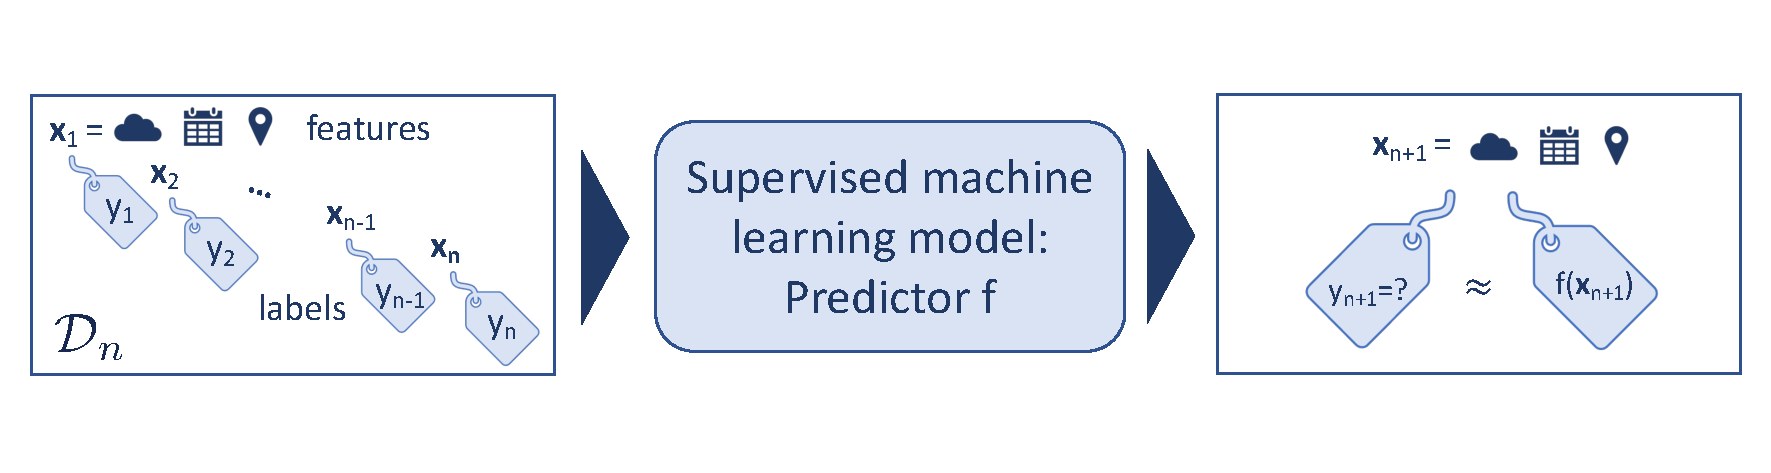
\includegraphics[width=0.9\textwidth]{figures/4-ml/machine learning.pdf}
    \caption{Illustration of the core principle of supervised learning.}\label{fgr:supervised_leaning}
\end{figure}

To do so, the learning algorithm uses a ``predictor'' $f$ that can be defined as the function that associates values (features) from $\mathcal{X}=\mathbb{R}^{p}$ to values of $\mathcal{Y}$. By changing the learning model (subsection~\ref{sct:model}) or by changing the feature space $\mathcal{X}$ we can define different domains $\mathcal{F}\subseteq{\mathcal{Y}}^{\mathcal{X}}$ where we search for the prediction function $f$. The domain $\mathcal{F}$ can either be too restrictive and the optimum function found is too far from the theoretical one, or be too large and the optimization problem is nearly impossible to solve or the solution is way too close to the data, which raises question of fitting that will be discussed later.

This predictor can be interpreted as the function that gives the most probable outcome $y$ for a given input $\mathbf{x}$. To evaluate the quality of the predictor, we can introduce a loss function $\mathcal{L}:\mathcal{Y}\times\mathcal{Y} \rightarrow \mathbb{R}^{p}$ that compares the predicted value $f(\mathbf{x})$ to the true value $y$ on the dataset at our disposal $\mathcal{D}_{n}$. This loss function needs to increase when $f(\mathbf{x})$ moves away from $y$. To extend the definition of the loss to the entire possible space, we can introduce the theoretical risk $\mathcal{R}$ of a predictor $h$ using the random variables $X$ and $Y$ so that $\mathcal{R}(h) = \E{\mathcal{L}\left(h(X),Y\right)}$. However, since we do not know the exact mapping of the random variables, we will rather evaluate empirically the risk $\mathcal{R}_n$ on the known dataset $\mathcal{D}_{n}$:
\begin{equation}\label{eq:risk}
  \mathcal{R}_n(h) = \frac{1}{n}\sum_{i=1}^n \mathcal{L}\left(h(\mathbf{x}_i),y_i\right)
\end{equation}

The goal is therefore to find a function that minimizes the risk function across the known data, and this optimal predictor $f^*$ can be defined as:
\begin{equation}\label{eq:min_f}
  f_n^* = \underset{f\in\mathcal{F}}{\text{arg min}} \mathcal{R}_n(f)
\end{equation}


Many loss functions can be used and depending on the definition, we emphasize more or less on the large errors. For instance, a quadratic cost function will penalize a lot the outlier so that a few medium errors are better than one great error, which is not the case for an absolute cost. Since I only used regression models for this thesis work, I will not go into the details of classification loss functions and will rather focus more on the regression loss functions. The quadratic loss or squared error loss $\mathcal{L}\e{SE}(f(\mathbf{x}),y)=0.5{\left(y-f(\mathbf{x})\right)}^2$ of a predictor $f$ on a data point $(\mathbf{x},y)$ is simply defined as the squared difference between the prediction and the true label. The multiplicative $0.5$ coefficient is here to simplify in the derivatives. This loss is similar to the mean squared error (MSE) used to compare two quantities across a dataset, the risk function actually corresponds to half of the MSE on the predictions $\mathcal{D}_n$:
\begin{equation}
  \mathcal{R}\e{SE}(f) = 0.5\frac{1}{n}\sum_{i=1}^n {\left(y_i-f(\mathbf{x}_i)\right)}^2
\end{equation}

A second very common loss function is the absolute loss, which is associated with the mean absolute error (MAE) used in error evaluation. The loss can be expressed as $\mathcal{L}\e{AE}(f(\mathbf{x}),y)=\left|y-f(\mathbf{x})\right|$, and the risk function associated is simply the MAE across the dataset predictions:
\begin{equation}
  \mathcal{R}\e{AE}(f) = \frac{1}{n}\sum_{i=1}^n \left|y_i-f(\mathbf{x}_i)\right|
\end{equation}
It is also possible to make this loss function flatter near the minimal error by introducing a parameter $\epsilon$. The $\epsilon$-insensitive loss corresponds to a modified absolute loss $\mathcal{L}_{\epsilon}(f(\mathbf{x}),y)=\max\left(0,\left|y-f(\mathbf{x})\right|\right)$.

Finally, it is possible to combine the less outlier-sensitive absolute loss with the smoothness of the quadratic loss near the minimal error domain by using a Huber loss. For a given $\delta$, the Huber loss is defined as:
\begin{equation}
  \mathcal{L}_{\delta}(f(\mathbf{x}),y) = \left\{
    \begin{array}{ll}
        \tfrac{1}{2}{\left(y-f(\mathbf{x})\right)}^2 & \mbox{for } \left|y-f(\mathbf{x})\right| \leq \delta \\
        \delta\left(\left|y-f(\mathbf{x})\right| - \tfrac{1}{2}\delta\right) & \mbox{otherwise.}
    \end{array}
  \right.
\end{equation}
And a risk function $\mathcal{R}_{\delta}$ can also be determined using this loss function. The Huber loss is considered as a robust loss function since it is less sensitive to the outliers (high values of error) and it has a very smooth gradient near the low values of error like the squared error. It can be seen as a combination of the advantages of both the absolute and squared errors as illustrated by the Figure~\ref{fgr:loss_comp}.

\begin{figure}[ht]
  \centering
    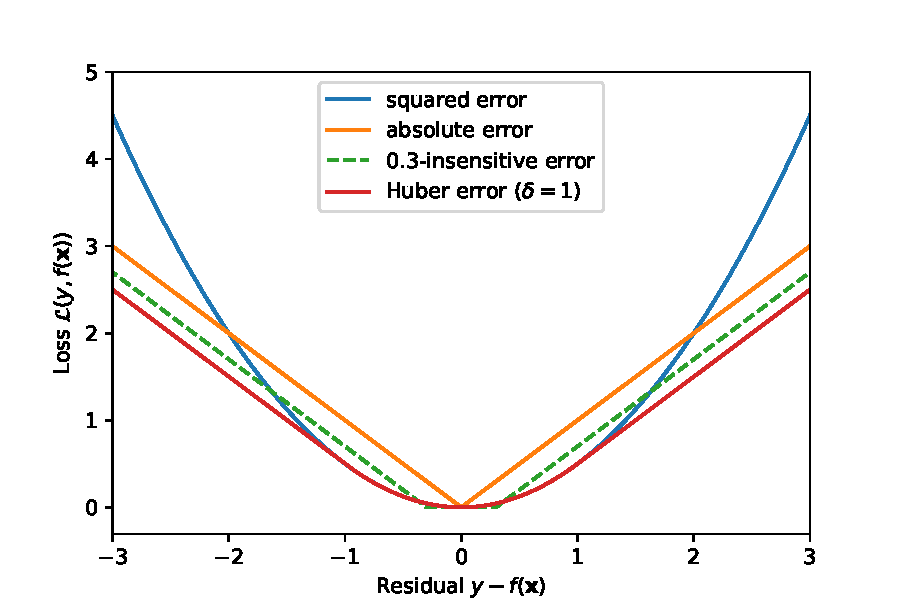
\includegraphics[width=0.6\textwidth]{figures/4-ml/loss_comparison.pdf}
    \caption{Comparison of different loss functions (quadratic loss, absolute loss, $\epsilon$-insensitive and the Huber loss). }\label{fgr:loss_comp}
\end{figure}

Through these theoretical considerations, I hope the process of a machine learning from data was demystified by simply formulating this leaning process as an optimization of a cost function, which is a common tool in any scientific field. However, this optimization problem is challenging in the sense that the variable is a function that lies in a high dimension space and approximations are needed to reduce the space. This is why most of the engineering breakthrough happens in the conception of the architecture of the ML model that defines the form of the prediction function $f$. Another difficulty of machine learning is to deal with an ill-posed problem, which means that one of the three conditions of Hadamard is not verified. These conditions being the existence and unicity of a solution and its continuity  with regard to the initial conditions. This issue is usually tackled using regularization techniques such as the one introduced by Tikhonov in the second half of the 20\e{th} century. Furthermore, the minimization of the empiric risk is not always consistent with the minimization of the more global risk (considering all possible observations), since minimizing $\mathcal{R}_n$ does not always give the same solution as the minimization of $\mathcal{R}$. Therefore, the complexity of the risk optimization problem depends on the loss function chosen but also the domain $\mathcal{F}$ defined by the model and different techniques can be used to construct a solution without anything that guarantees the optimality of it. One of the biggest challenges of ML is to overcome the problem of generalizability, which will be the topic of the next discussion.


\subsubsection{Generalization and overfitting}

As previously discussed, the optimization problem is ill-defined and we have no guarantee for the model to work on other data points as $n$ goes toward infinite. The generalizability of model consists in ensuring the predictability of unseen data so that the solution does not simply correspond to the minimal risk for the data $\mathcal{D}_{n}$ but also for other $m$ data points $\left\{(\mathbf{x}_{n+1},y_{n+1}),\ldots,(\mathbf{x}_{n+m},y_{n+m})\right\}$ all different from the previous set. One of the main phenomena that explain this discrepancy between the solution $f_n^*$ and the ideal solution $f^*$ (considering an infinite amount of data) is the noise in the dataset. The data is not perfectly measured, and the uncertainty attached to each $\mathbf{x}_i$ and $y_i$ values can create a residual noise that needs to be ignored in the learning process. Moreover, sometimes, the $p$ explanatory variables considered are not enough to model the target phenomenon. To train a generalizable model, we would need to learn enough to capture the inner relation between $X$ and $Y$, but it should not fit the data too closely and capture the noise along the way, otherwise we say that the model overfits the data. If the model is very inaccurate even on the training data, we say that the model underfits, and generally it means that the model is too simplistic (not enough features or too low-level architecture). 

This problem of overfitting can be summarized in the fundamental notion of bias--variance tradeoff in machine learning and more generally in statistics. The error can be broken down in two types: the bias error measures the error made on the available data $\mathcal{D}_n$, while the variance error measures the sensibility to small variations in the input values. A high bias error corresponds to an underfitting, we did not learn enough from the data; and a high variance error means an overfitting, we learned too much even superfluous relations. To formalize these errors, we can go back to the empiric risk function $\mathcal{R}_n(f)$ that models the error of our predictor $f\in\mathcal{F}$; to know if we reach the ideal optimum we would need to compare it to the minimal risk that a predictor with infinite knowledge would get $\mathcal{R}^* = \underset{\scriptscriptstyle h\in\mathcal{Y}^{\mathcal{X}}} {\text{min}}\mathcal{R}(h)$. This excess error $\mathcal{R}_n(f)-\mathcal{R}^*$ can then be broken down in two errors that could be interpreted as the bias and the variance errors:
\begin{equation}\label{eq:generalization_error}
  \mathcal{R}_n(f)-\mathcal{R}^* = \left[\mathcal{R}_n(f) - \underset{\scriptstyle h\in\mathcal{F}} {\text{min}}\mathcal{R}_n(h)\right] + \left[\underset{\scriptstyle h\in\mathcal{F}} {\text{min}}\mathcal{R}_n(h) -\mathcal{R}^*\right]
\end{equation}
The first term of the above-written sum corresponds to a bias error, because it measures how far the current predictor $f$ is off of a minimum (there can be several in an ill-posed problem) risk predictor $f_n^*$ determined using the $n$ data points. The second term, on the other hand, is the residual error associated with the choice of the predictor domain $\mathcal{F}$ and the fact that only a finite amount of data is accessible to the prediction model. With an infinite amount of data, the model $f^*$ associated with the risk $\mathcal{R}^*$ would not be influenced by the noise since several data points with similar features but with small noises would give a similar prediction. The difference of loss between this ideal function $f^*$ and the current function we are testing $f$ would correspond to an overfitting of the noise that could not be distinguished in the finite case, if we consider the domain $\mathcal{F}$ defined by the model suitable. On the contrary, if there is a problem of model, this error also measures the approximation error due to the choice of a given set of features with a given model architecture.

\begin{figure}[ht]
  \centering
    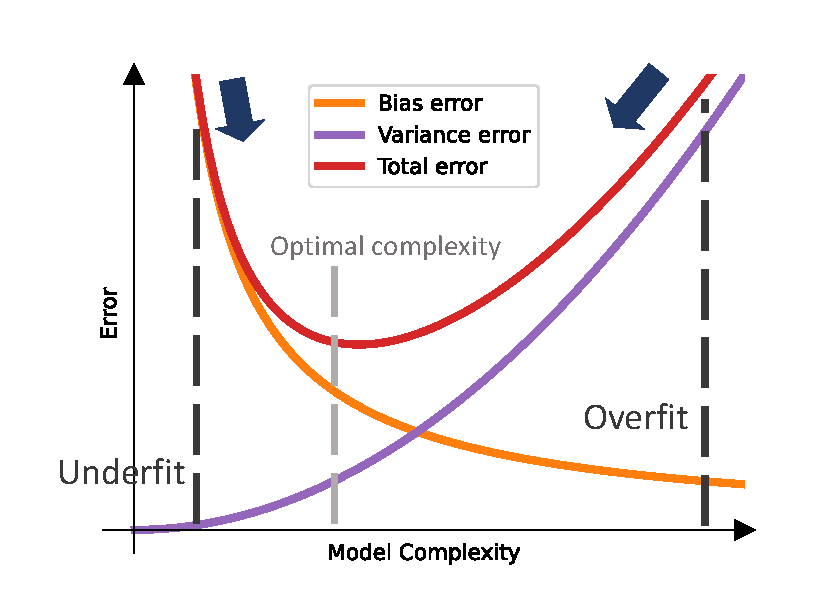
\includegraphics[width=0.45\textwidth]{figures/4-ml/Bias_variance_tradeoff.pdf}
    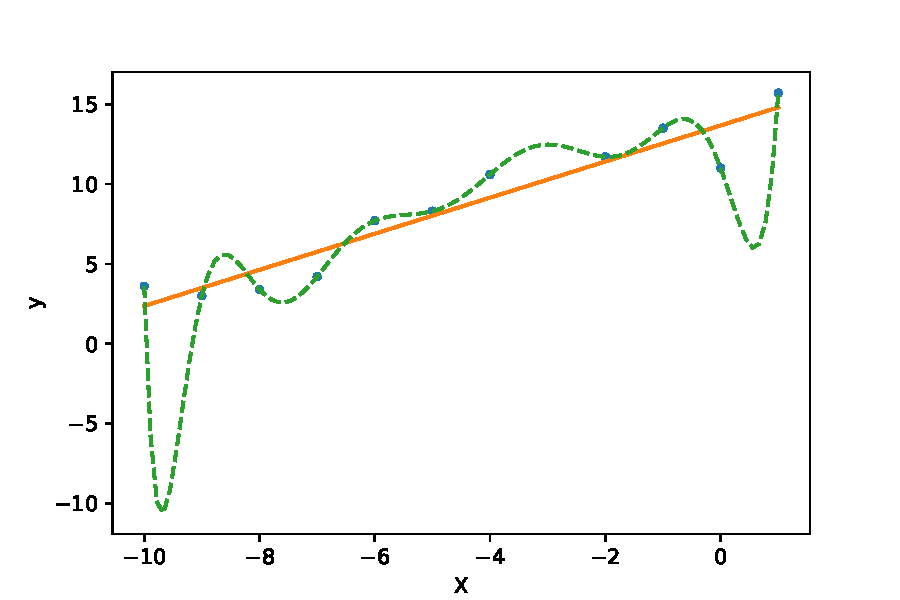
\includegraphics[width=0.45\textwidth]{figures/4-ml/overfit.pdf}
    \caption{On the left, theoretical relation between the bias, variance and total errors and the model complexity. The overfit case is illustrated on the right plot when considering polynomial fits. The lower degree linear function is more generalizable than the biased high degree polynomial that fits perfectly the data.}\label{fgr:bias_variance}
\end{figure}

In general, if the model is very complex in comparison to the amount of data we have, we would fit too closely to the data and have a very high change to overfit. The opposite is also true, a simplistic model would yield to a poor bias error and the model would be underfit. This principle is represented on the Figure~\ref{fgr:bias_variance} and should guide us in the design of a new ML model.
The complex art of fitting a model to a dataset consists in finding the right balance between the bias and the variance. Fortunately, some optimization tools can help us reduce the variance error by changing the loss function itself, and I will introduce them in the next part of our discussion.

\subsubsection{Regularization to fight against overfitting}

Regularization consists generally in adding implicit or explicit constraints on the optimization problem to find not only the most accurate solution (minimal loss) but also the simplest. This criterion of simplicity is crucial in the generalization of the problem. We typically don't need a high degree polynomial when a linear function is a more suitable solution as shown on Figure~\ref{fgr:bias_variance}. 

The explicit regularization technique consists in penalizing the complexity of a model by adding to the global loss function an error term that scales with the complexity of the model. The error associated to a predictor $f$ can be expressed with an additional regularization term ${\Omega}_n(f)$:
\begin{equation}
  \mathcal{R}_n(f) = \frac{1}{n}\sum_{i=1}^n \mathcal{L}\left(f(\mathbf{x}_i),y_i\right) + \Omega_n(f)
\end{equation}
And, depending on the expression of the regularization term ${\Omega}_n(f)$, the regularization will have more or less influence on the optimization problem. 

Since the regularization is a model-specific function (depends on $f$), we need to define a model to study more specific expressions of regularization. 
Let's consider a multilinear model so that $f(\mathbf{x}) = \boldsymbol{\beta}\mathbf{x}\ex{T}$, where $\boldsymbol{\beta}=(\beta^{(1)},\ldots,\beta^{(p)})$ is a vectorial representation of the weights of the $p$ features contained in $\mathbf{x}$ in the linear regression. In a standard multilinear regression, with a quadratic loss, the risk function to minimize can be expressed as:
\begin{equation}\label{eq:linear}
  \mathcal{R}_n(f) = \frac{1}{n}\sum_{i=1}^n {\left(\boldsymbol{\beta}\mathbf{x}_i\ex{T}-y_i\right)}^2 
\end{equation}
and $y_i$ is now a scalar in a regression problem ($\mathcal{Y}=\mathbb{R}$). One of the earliest regularization tools introduced by Tikhonov to deal with ill-posed optimization problem is the L2 regularization. Used in linear regression, this new type of model is called the ridge regression and consists simply in adding a L2-norm penalty on the model weights in the risk function as expressed in the following equation:
\begin{equation}\label{eq:L2_reg}
  \mathcal{R}_n(f) = \frac{1}{n}\sum_{i=1}^n \mathcal{L}\left(f(\mathbf{x}_i),y_i\right) + \lambda_2 {\lVert \boldsymbol{\beta} \rVert}_2^2 = \frac{1}{n}\sum_{i=1}^n {\left(\boldsymbol{\beta}\mathbf{x}_i\ex{T}-y_i\right)}^2 + \lambda_2 \sum_{k=1}^p \left|\beta^{(k)}\right|^2
\end{equation}
where $\lambda_2$ is the parameter of the L2-regularization, it controls the importance of the regularization term in the optimization process. This parameter controls the complexity of the model and needs to be tweaked to find the optimum between accuracy and generalizability as shown on the Figure~\ref{fgr:bias_variance}. If we now consider a polynomial function, the vector $\mathbf{x}_i$ represents the vector of different exponentiations of a scalar $x_i$ so that $\mathbf{x}_i=\left(x_i^0,\ldots,x_i^{n-1}\right)$, and the coefficients $\boldsymbol{\beta}$ are just the polynomial coefficients of the polynomial function $f$. This is a clear illustration of how the complexity of the model is penalized since regularization terms directly penalize the number of terms used and their influence on the fitting process.
Note that this regularization can be adapted to other types of models, given that we manage to define a L2-norm of the prediction function $f$.

A second very common regularization term is based on the L1-norm of the prediction function. A L1-regularized least square linear regression is called a LASSO (Least Absolute Shrinkage and Selection Operator) regression, it allows for a sparser selection of the model weights by allowing zero weights in the model, which is not the case for a L2-regularization. The risk function associated with this regression model can be expressed as:
\begin{equation}\label{eq:L1_reg}
  \mathcal{R}_n(f) = \frac{1}{n}\sum_{i=1}^n \mathcal{L}\left(f(\mathbf{x}_i),y_i\right) + \lambda_1{\lVert \boldsymbol{\beta} \rVert}_1 = \frac{1}{n}\sum_{i=1}^n {\left(\boldsymbol{\beta}\mathbf{x}_i\ex{T}-y_i\right)}^2 + \lambda_1 \sum_{k=1}^p |\beta^{(k)}|
\end{equation}
where $\lambda_1$ is the L1-regularization parameter that controls its importance. The L1-norm can be defined differently depending on the model, but the core idea is that it is a function of the absolute values of the weights of the model. 

Finally, if we combine both L1 and L2-regularization, the linear regression becomes an elastic net regression and the risk function becomes:
\begin{equation}\label{eq:elasticnet_reg}
  \mathcal{R}_n(f) = \frac{1}{n}\sum_{i=1}^n \mathcal{L}\left(f(\mathbf{x}_i),y_i\right) + \lambda_{1,2} \left({\alpha \lVert \boldsymbol{\beta} \rVert }_1 + (1-\alpha) {\lVert \boldsymbol{\beta} \rVert}_2^2\right)
\end{equation}
where $\alpha\in[0,\,1]$ defines the relative weight of L1 and L2 regularization term and $\lambda_{1,2}$ governs the importance of the combined regularization term. This regularization technique simply combines both L1 and L2 regularization, and the different regularization parameters can be tweaked to find the best bias--variance tradeoff for the final model. These parameters are also called hyperparameters in machine learning, because it changes the parameters at the higher model level.

Finally, implicit regularization corresponds to other forms of control of the complexity of the model. For instance, it could be the early stopping in a learning process so that we do not converge completely to the minimal error with the data. It could be discarding outliers that prevent the model from learning properly on the relevant data. It could also be in the architecture of the model, for instance the random forest is an ensemble approach that aims at reducing the overfit, and it will be presented in the next section. The learning rate in the gradient boosting is also a regularization parameter that smoothes the learning process and will be tackled in the dedicated section. The implicit regularization is related to the construction of the model itself and will therefore be explained in more details in the section on machine learning models.

\subsubsection{Learning strategies}

I previously introduced the theory behind the bias--variance tradeoff, which boils down to the generalization of model that has a partial glimpse of all the available data. Yet, in practice we need to evaluate the generalization error $\mathcal{R}_n(f)-\mathcal{R}^*$. To achieve that, the common strategy is to randomly split the available data into two sets a training set $\mathcal{D}\ex{train}=\left\{{(\mathbf{x}_{i_1},y_{i_1}),\ldots,(\mathbf{x}_{i_N},y_{i_N})}\right\}$ and a test set $\mathcal{D}\ex{test}=\left\{(\mathbf{x}_{j_1},y_{j_1}),\ldots,(\mathbf{x}_{j_{n-N}},y_{j_{n-N}})\right\}$ so that $\mathcal{D}_n = \mathcal{D}\ex{train} \cap \mathcal{D}\ex{test}$. The training set is used to perform the optimization problem as defined in equations~\ref{eq:risk} and~\ref{eq:min_f}, and the test set is used to evaluate the generalization error since it is unseen data for the model. In practice, we choose a ratio of test data $n-N/n$ (e.g.\ {20\%}) that defines the size of the test set from an initial dataset, and the randomness of the split ensures that the data from both sets are similar yet not exactly the same. However, in some cases, one should be aware that outliers can be present in the test set, which makes the performance on the test set worse than expected. Or in some cases, the dataset is too small and every data point is very different from each other, and the test set is very different from the training set, which makes it impossible for the model to predict on the test with the piecemeal information given by the training set. The percentage of the train/test split should therefore be chosen wisely and according to the dataset so that it remains representative of the training set.

The main property of the test set is that it is a completely unsee dataset, which means that the training of the model should be independent of this set except for the very final evaluation. But in some cases, we want to compare different models with each other or change a ``hyperparameter'' like the regularization parameter within the same model architecture. To evaluate these models, we cannot evaluate for every model the generalization error on the test set, because it would compromise the independence of the test set with the training process. Hence, we introduce validation sets within the initial training set. We could do a simple training/validation split similar to the train/test split. However it would weaken the model even more since there is less data available, and, furthermore, it does not use all the potential of the training set. A very common technique to test the performance of a model on a training set is the cross-validation. The idea is to use different training/validation splits to test the model in multiple configurations to have a better evaluation of the model performance by averaging the different performances. 

The most used method is the k-fold cross-validation technique which consists in partitioning the training set $\mathcal{D}\ex{train}$ in k equal size subsets $\mathcal{S}_1,...,\mathcal{S}_k$. The model is then trained on the union $\bigcup_{l\neq m} \mathcal{S}_l$ of all subsets but one subset $\mathcal{S}_m$ that will be used as a validation set for all $m\in \{1,\ldots,k\}$. The principle of the k-fold approach is illustrated on the Figure~\ref{fgr:kfold}. The approximate generalization error of the model is then the average of every loss calculated on the validation subsets. This tool provides a way of comparing different models without using the test set, which is extremely useful especially in the parameterization of the ML model.

\begin{figure}[ht]
  \centering
    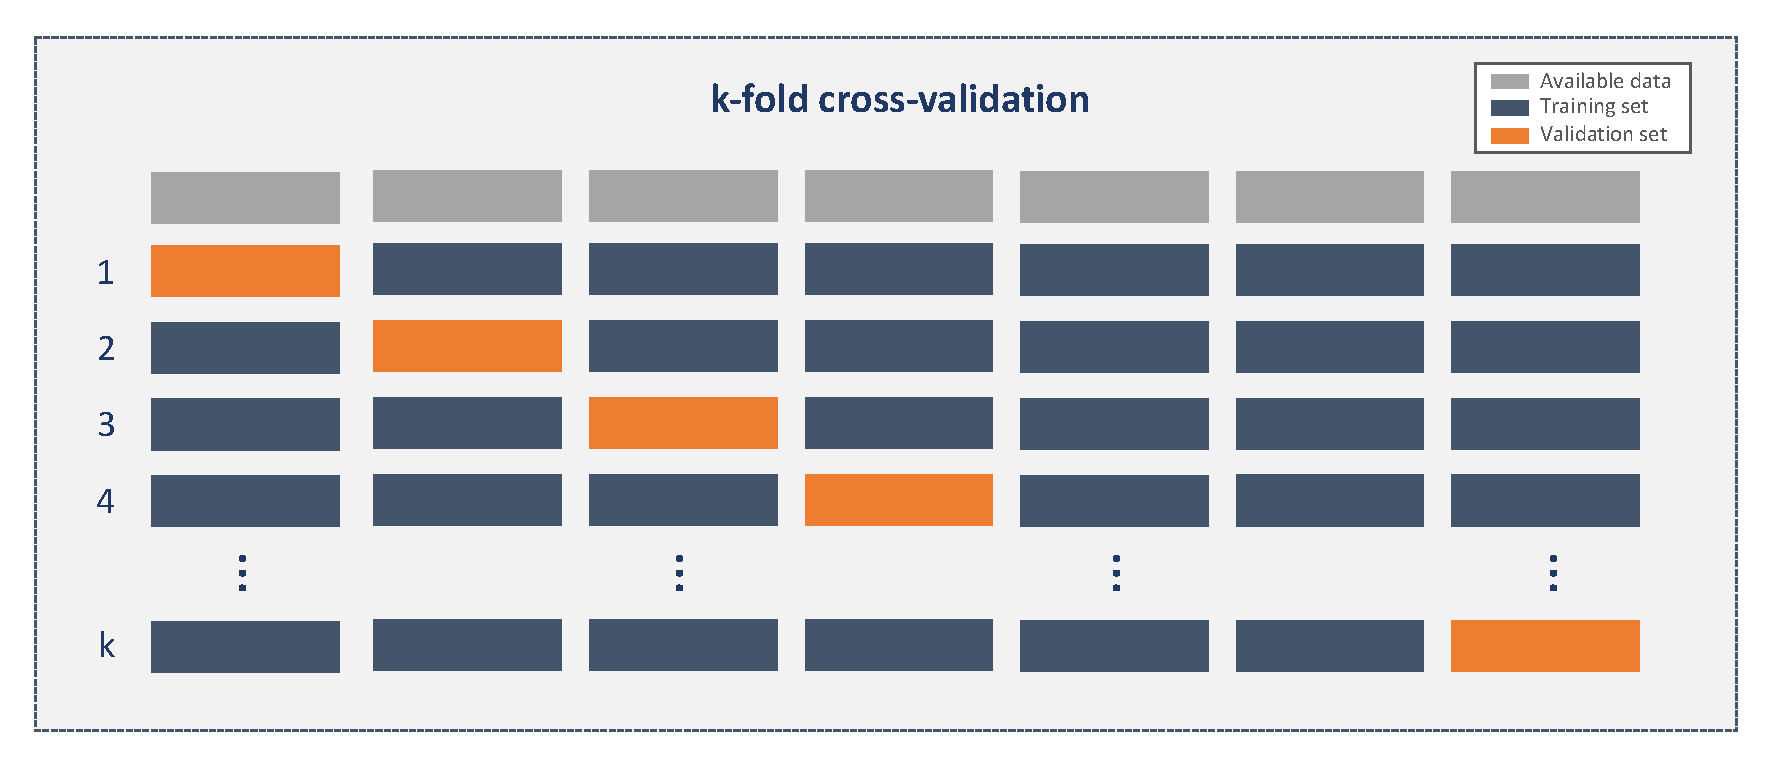
\includegraphics[width=0.8\textwidth]{figures/4-ml/cross-validation.pdf}
    \caption{Illustration of a k-fold cross-validation. At each step, the machine learning model learns from the training set and is tested on the validation set. The average performance on all validation sets gives an approximation of the generalization error.}\label{fgr:kfold}
\end{figure}

Other cross-validation techniques exist and are used in specific cases, for example the stratification cross-validation consists in ensuring the same repartition of the labels $y_i$ in each subset, which is useful in classification problems. We can also make the validation process even more exhaustive by increasing the k in the k-fold validation. However it requires k training of the models, which increase the computation time required. When increase to the maximum k is equal to the size of the training set and the method is called leave-one-out cross-validation. Finally, for time series, the cross-validation technique usually requires to sort the data according to the time history so that the training set is always prior to the validation set, which creates a whole new approach to cross-validation. The core idea of cross-validation is to find multiple training/validation splits to evaluate the model from more than one point of view, and different strategies exist depending on the training problem before us.

\subsection{Machine learning models}\label{sct:model}

In this chapter, I will go from the basic components of the model (decision tree) to the more complex ensemble model (e.g.\ random forest), in order to finish with the final stochastic gradient boosting model I used in this work. The discussion will be mainly focused on regression problems and not classification problems since the goal is to predict a continuous variable (the xenon/krypton selectivity).

\subsubsection{Regression tree}

Tree-based models are usually used in classification problems where depending on a set of ``yes'' or ``no'' questions the tree classifies the data points into the different predefined categories. The questions are in fact associated to threshold values of the $p$ features or characteristics $C_1,\ldots,C_p$; for example, a node of the tree could ask the question, ``Is $C_1$ higher than $3$?'', which splits the space into two categories the ``yes'' and the ``no''. This is why we can see a decision tree model as a splitting of the space into rectangles (in 2D) or an equivalent of a rectangle in $p$-dimensional feature space. To adapt this type of model into a regression problem, we can regroup different label values $y$ into categories that are represented by the average label value. To sum up, a decision tree for regression splits the feature space into a set of pseudo-rectangles (volumes separated by limited hyper-surfaces) defined by the nodes of the tree, and in each of these subspaces are given the average of the different points present in this subspace. To clarify the terminology, a splitting node correspond to a separation between regions, while a terminal node or leaf corresponds to the region itself.

\begin{figure}[ht]
  \centering
  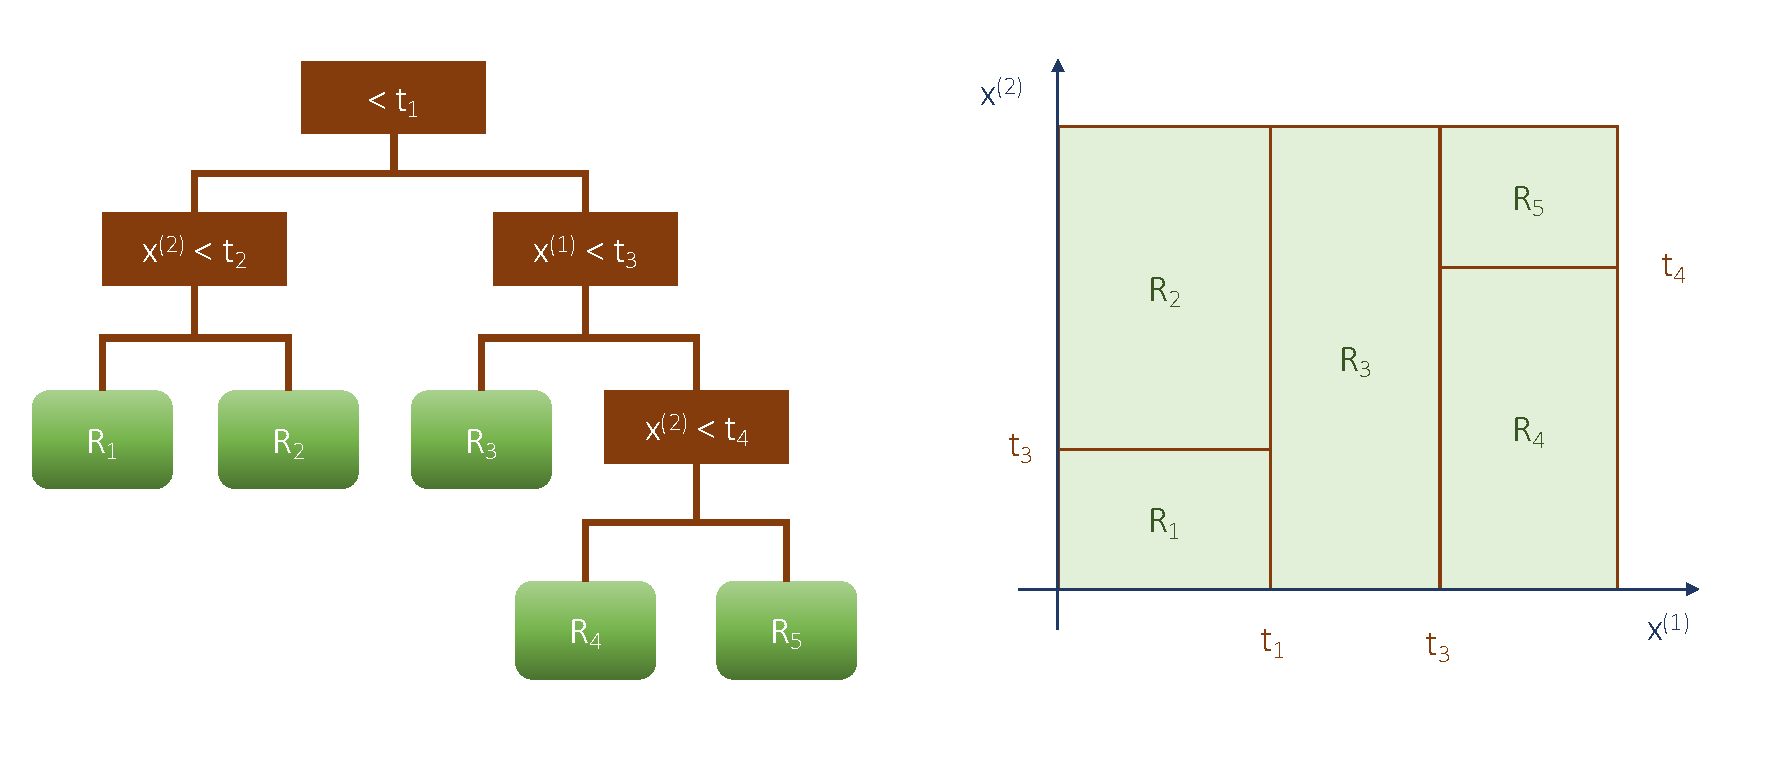
\includegraphics[width=0.8\textwidth]{figures/4-ml/decision_tree.pdf}
  \caption{Illustration of the decision tree and the region splitting performed by a CART\autocite{Breiman_2017} algorithm. Adapted from an illustration of the book ``Elements of Statistical Leanrning''~\cite{Hastie_2009}.}\label{fgr:tree}
\end{figure}

The CART\autocite{Breiman_2017} algorithm developed by Breiman et al.\ is usually presented as the archetype of a decision tree model. The algorithm is pretty straightforward to understand, three steps are required: (i) Examine every split allowed on each feature $C_i$, (ii) select and use the best split according to a loss function (squared error or absolute error usually), and (iii) stop splitting a node when a stopping rule is satisfied (e.g.\ minimum samples split).\autocite{Dension_1998} We could split indefinitely the decision tree so that each data point has its own region, but this would be a textbook case of overfitting, any new data point would never be correctly predicted with such a model. To prevent this from happening, the decision tree has a regularization parameter called minimum samples split $n\e{min}$ that only allows a further split; if the node contains less than a given number $n\e{min}$, then it is necessarily a terminal node. The decision trees are known to be very prone to overfitting, another useful regularization parameter can be used to prevent an ever-growing tree is the maximum depth of the tree,  which can also stop the iterative process of tree growing. Finally, to further regularize the tree, a process called tree pruning simplifies the tree and outputs the final model. I won't go into the details of tree pruning as it is not the main subject (see Ref.~\cite{Hastie_2009} for further details). The final tree $f\e{tree}$ can be expressed as a function of the different regions $R_1,\ldots,R_M$ carved by the splitting process:
\begin{equation}
  f\e{tree}(\mathbf{x}) = \sum_{m=1}^M c_m \mathbb{1}(\mathbf{x}\in R_m)
\end{equation}
where $c_m$ is the value of the leaf corresponding to $R_m$, and $\mathbb{1}$ is an identity function that returns $1$ if the argument is true and $0$ otherwise. The coefficients $c_m$ of this function are actually equal to the average of the labeling values of the dataset $\mathcal{D}_n$ in the region $R_m$, i.e. $c_m= \underset{i\in \mathcal{D}_n}{\text{ave}}(y_i|\mathbf{x}_i\in R_m)$.
To put it simply, the tree function returns the average value of $y$ (in the dataset) in the region where $x$ (could be new data) is located. 

The decision tree has the main advantage of being very easily interpretable as defined in the book of C. Molnar~\cite{molnar2020interpretable}. This interpretability boils down to the easily understandable binary decision at the root of the decision tree --- we can easily see the explaining characteristics ($R_m$) of a predicted value, we can easily imagine different predictions depending on the value of $\mathbf{x}$, and for small trees we can even run the model in our own head. However, this model has a reputation of being very inefficient in finding simple linear relations resulting in a step-like function. The model is not very smooth, slight changes in the input $x$ can have a big impact on the predicted value (typically near the separation between two regions) and some change (noise) in the training data can totally change the structure of the tree. This instability of a single tree makes it very hard to generalize over unseen data.\autocite{molnar2020interpretable} To improve this single decision tree, Breiman introduced bagging predictors in 1996 to improve the accuracy of models that are unstable with regard to small changes in the learning set.\autocite{Breiman_1996} This new approach is at the origin of the random forest, and will be presented more in depth in the following subsection.

\subsubsection{Random Forest}

The core idea behind random forest is that a collection of weak learners, called an ensemble model, is better than a single strong learner, this assumption relies on a proven theorem that states that the minimal error of a forest is lower than the error of a single tree (theorem 11.2.\ of Ref.~\cite{Breiman_2001}). The strength of a model depends on the amount of information we feed into the model and its complexity. To achieve a diverse forest of weaker decision trees, we need to introduce two concepts; the first one is the bootstrap aggregating (bagging) and second one is the random column subsampling. Both methods ensure a diversity in the generated trees by using random selections and also a relative weakness of the trees by reducing the amount of information it can access. 

The bagging method consists in generating a set ${\left\{\phi_b\right\}}_{b\in \{1,\ldots,B\}}$ of $B$ weaker learners from different bootstrap datasets ${\left\{\mathcal{D}\ex{train}_b\right\}}_{b\in \{1,\ldots,B\}}$. Each bootstrap dataset $\mathcal{D}\ex{train}_b$ is generated by randomly selecting $t$ elements of $\mathcal{D}\ex{train}$ using a sample with replacement --- note that each bootstrap sample has the same number of elements than $\mathcal{D}\ex{train}$ but data points can appear several times in it. The number of times a data point $(\mathbf{x}_i,y_i)$ appears represents the weight of this data point in the bootstrap learning set. To simplify, we can say that each tree model $\phi_b$ learns on the $\mathcal{D}\ex{train}_b$ dataset that have randomly defined weights on the different data points, which means that every model will pay attention to different parts of the training data. We can also evaluate the generalization error of the model since some trees have never seen some data points, we can evaluate the generalization error on the unseen data for every tree (similar to cross-validation), this error is called the out-of-bag error.

The second technique consists in randomly choosing a subsample of the features on which to find the best split (second part of the CART tree growing algorithm). This technique is inspired from the one developed by Ho in 1998, where each tree of a forest is trained only on a randomly chosen feature subspace.\autocite{Tin_Kam_Ho_1998} The only tweak in the procedure lies in the fact that the feature space changes at each iteration of the tree growing process instead of between each tree generation. This method also improves the generalizability of the method by weakening each tree so that they don't overfit, the accuracy is achieved by the aggregation of all the trees. 

The random forest as formulated by Breiman combines these two randomness-based techniques to train a forest.\autocite{Breiman_2001} The algorithm starts by looping over the number of trees $B$ in the forest, for each tree $b$ a bootstrap sample $\mathcal{D}\ex{train}_b$ is randomly drawn (with replacement) and this data is used to grow the tree (training procedure). In the training, a modified CART algorithm is applied to grow the tree by splitting recursively on each node: (i) instead of testing all features for the best splitting, only a random selection of $m$ variables is considered among the $p$ features, (ii) the best split point is selected among the $m$ variables, and (iii) the node is split in two until the minimum leaf size $n\e{min}$ is reached. The size of the column subsample defines the number of features to randomly consider at each split; this is another implicit regularization parameter associated with the random forest along with the previously identifies regularization parameters of the decision tree such as the minimal leaf size $n\e{min}$ or the maximal depth of a tree. Finally, we have a set of $B$ trees $\left\{\phi_b\right\}$ that can be used to make an ensemble model $\Phi$ so that:
\begin{equation}
  \Phi(\mathbf{x}) = \frac{1}{B}\sum_{b=1}^{B} \phi_b(\mathbf{x}) = \frac{1}{B}\sum_{b=1}^{B}\sum_{m=1}^{M_b} c_{m,b} \mathbb{1}(\mathbf{x}\in R_{m,b})
\end{equation}
Note that each tree has an equal amount of say in the prediction, and they are trained on different random samples of the initial training data. Random forest is known to be less prone to overfitting because it is the produce of a sort of cross-validation process called bootstrapping. However, the algorithm does very little improve the accuracy (bias error) of the model it relies on the belief that each tree will naturally compensate their mutual weaknesses in the final ensemble model. In the next section, I will introduce another algorithm that focuses on guiding each tree based on the prior knowledge of previous trees to perform better --- this new technique is called boosting.

\subsubsection{From boosting to gradient boosting}\label{sct:boosting}

In the previous approach, the bootstrap dataset is a random selection of the samples in the training set $\mathcal{D}\ex{train}$ and each tree has an equal vote in the final ensemble decision. In a boosting algorithm,\autocite{drucker1997improving} the paradigm changes, data samples are (i) selected according to how they were predicted by the previous trees in order to focus our attention on the poorly predicted sample points, and (ii) the tree $\phi_b$ that is trained on this weighted dataset $\mathcal{D}\ex{train}_b=\left\{\left(w_i^{(b)},\mathbf{x}_i,y_i\right)\right\}$ is also evaluated using a measure of confidence $\alpha_b$ that depends on the error made (the higher the error, the lower the confidence), this measure of confidence is used to define the ensemble model:
\begin{equation}
  \Phi_B = \frac{1}{\sum_{b=1}^{B} \alpha_b}\sum_{b=1}^{B} \alpha_b\phi_b
\end{equation}

To train each individual tree $\phi_b$ of this forest, we use the CART algorithm (described in the previous sections), but by minimizing a weighted risk function instead of the standard one:
\begin{equation}
  \mathcal{R}(\phi_b) = \sum_{i=1}^N w_i^{(b)} \mathcal{L}\left(\phi_b(\mathbf{x}_i),y_i\right)
\end{equation}
where $w_i^{(b)}$ is the normalized weight corresponding to the error $\mathcal{L}\left(\Phi_{b-1}(\mathbf{x}_i),y_i\right)$ made by the previous ensemble $\Phi_{b-1}$ on each data point $\left(\mathbf{x}_i,y_i\right)$; for $b=1$, there is no previous model so the weights are just equidistributed across the samples, i.e. $\forall i,\ w_i^{(1)}=1/N$. In practice, to simulate the weighting process, a random selection with probability $w_i^{(b)}$ on each sample is performed to draw an equal-sized $N$ training dataset $\mathcal{D}\ex{train}_b$ for $\phi_b$. 

I voluntarily did not go into the details of the confidence rate $\alpha_b$, because several implementations of it exist. But generally, it is a decreasing function of the total error of the tree on the weighted dataset. The AdaBoost algorithm typically uses the half the opposite of the logit transform function $\alpha_b=0.5\log\left((1-\mathcal{R}(\phi_b))/\mathcal{R}(\phi_b)\right)$ that goes to $+\infty$ for very small errors and $-\infty$ for very large ones.\autocite{Freund_1997,schapire2013explaining} Gentle AdaBoost would give an equal amount of say to each tree independently of their performance, which can in some cases allow better generalization performance than a regular AdaBoost. The very high values of $\alpha_b$ could in some cases make the model overfit, because a very good performance on the weighted dataset could mean a good fit on noisy data points.\autocite{schapire1998improved} To prevent overfitting early stopping procedure with a cross-validation (k-fold usually) training procedure is performed to determine the ideal number of trees required to stay generalizable while having reduced the bias error --- like always in machine learning it is a question of bias--variance tradeoff. 

AdaBoost in its original implementation uses stamps which are trees composed of a unique splitting node and two leaves, but boosting algorithms can be applied to any tree depth. This tree depth hyperparameter is very important in tree-based models since it defines the complexity/strength of each learner tree. A smaller tree would usually overfit less (see link between complexity and variance on Figure~\ref{fgr:bias_variance}), and the AdaBoost algorithm uses the smallest possible tree in order to compensate the very aggressive learning procedure used. The main takeaway from this study is that boosting focuses on the training trees that compensate the errors of previous trees, and it can play with tree-based hyperparameters (e.g.\ tree depth, number of trees) to control the variance error.

Actually boosting can be reformulated as a gradient descent problem as formulated by Mason et al.\autocite{mason1999boosting} We can prove that AdaBoost is simply a gradient boosting algorithm with an exponential loss (same loss and derivative) and with the steepest gradient descent logic.\autocite{mason1999boosting,azencott2022introduction} 

Each additional tree $\phi_{b}$ in a gradient boosting can be interpreted as a contribution to a predictor $\Phi_{b}$ to minimize an objective function $\mathcal{R}(\Phi_{b})$. And the weight $w_i^{(b)}$ which measures how badly each sample $i$ are predicted, can be expressed as a derivative of a differentiable loss function $\mathcal{L}$ since the minimum is reached for a zero derivative. 
\begin{equation}
  w_i^{(b)} = -\left.\frac{\partial\mathcal{L}\left(y_i,\hat{y}_i\right)}{\partial\hat{y}_i}\right|_{\hat{y}_i=\Phi_{b-1}(\mathbf{x}_i)}
\end{equation}
where $\hat{y}_i$ is a derivation variable describing the ensemble tree prediction, here evaluated at $\Phi_{b-1}$. Instead of predicting the $y_i$ values, we can predict the weight, also called the pseudo-residual, $w_i^{(b)}$ that measures how far the previous model $\Phi_{b-1}$ is from the ideal $\Phi$ (zero weights everywhere in an ideal world) and compensate it using a tree $\phi_{b}$. In other words, we use the CART framework to grow a tree $\phi_{b}$ that predicts the gradients $w_i^{(b)}$ from the features $\mathbf{x}_i$, which iteratively improves the model $\Phi_b$ compared to $\Phi_{b-1}$: 
\begin{equation}
  \Phi_b = \Phi_{b-1} + \eta \phi_{b}
\end{equation}
where $\eta$ is the learning rate or shrinkage, introduced by Friedman in his stochastic gradient boosting, to slow down the learning process in order to limit overfitting.\autocite{Friedman2002} In a steepest descent step, the values of this learning rate $\eta$ actually minimizes the risk function $\mathcal{R}(\Phi_{b-1} + \eta \phi_{b})$ associated to the output model $\Phi_b$. If $b=1$, the first estimator $\Phi_1$ is simply a constant function that minimizes the risk over the training set $\Phi_1(\mathbf{x}) = \underset{c\in \mathbb{R}}{\text{arg min}} \sum_{i=1}^{N}\mathcal{L}(y_i,c)$. For a quadratic loss function, this constant corresponds simply to the average of the $y_i$ values over the training set.

In the particular case of a quadratic loss $\mathcal{L}\e{SE} =\tfrac{1}{2} {\left(y_i - f(\mathbf{x}_i)\right)}^2$ that is used in this chapter, the gradient boosting algorithm can be simply broken down into the three steps below:\autocite{Friedman2002}
\begin{enumerate}
  \item Initialization at $b=1$ with a constant: \\
    \quad $\Phi_1(\mathbf{x}) = \frac{1}{N}\sum_{i=1}^{N}y_i$
  \item For $b = 2$ to $B$:
    \begin{enumerate}
      \item Compute the pseudo-residuals that are actually real residuals in the case of a quadratic loss
        \quad $\forall i\in \{1,\ldots,N\},\ w_i^{(b)} = y_i - \Phi_{b-1}(\mathbf{x}_i)$
      \item Train the weak tree $\phi_b$ on the dataset ${\left\{ (\mathbf{x}_i, w_i) \right\}}_{i\in \{1,\ldots,N\}}$.
      \item Update the model using a fixed learning rate $\eta\in [0,1]$ instead of finding $\eta =\underset{c\in \mathbb{R}}{\text{arg min}} \sum_{i=1}^{N}\mathcal{L}\left(y_i,\Phi_{b-1}(\mathbf{x}_i) + c \phi_b(\mathbf{x}_i)\right)$ through a minimization problem (steepest gradient descent).
        \quad $\Phi_b = \Phi_{b-1} + \eta \phi_{b}$
    \end{enumerate}
  \item Output the final ensemble model $\Phi_B$
\end{enumerate}

Up until now, I showed the different ways of using decision trees to perform a prediction on a training dataset $\mathcal{D}\ex{train}$ by focusing on mainly two ensemble models: random forest and gradient boosted trees. The reason why I went through these models is to be able to present my prediction model that aggregates techniques from both ensemble models. This model, called eXtreme Gradient Boost or XGBoost, was introduced by Chen et al.\ and is an improvement compared to similar methodologies due to its scalability. I won't go into the details of the implementation improvement (for more details see Ref.~\cite{chen2016xgboost}), but I will rather focus on the basic framework it uses to better understand the core components of the model.

\subsubsection{XGBoost model parameterization}

The XGBoost model is basically a gradient boosting model as decribed in the previous section but with a few regularization parameters that could be fine-tuned to improve its generalizability. In a learning problem with $N$ learning examples and $p$ features/descriptors, we can express the predictor $\Phi$ as the sum of weaker tree learners $\phi_b$:
\begin{equation}
  \Phi(\mathbf{x}) = \sum_{b=1}^{B} \phi_b(\mathbf{x}) = \sum_{b=1}^{B} \sum_{m=1}^{M}c_m^{(b)} \mathbb{1}(\mathbf{x}\in R_m^{(b)})
\end{equation}
where $M$ is the maximal number of leaves a tree can have, in our implementation --- this number is fixed using the maximum depth $\max\e{depth}$ in the algorithm since $M=2^{\max\e{depth}}$, and $B$ is the maximum number of estimators in the ensemble model. The number of estimators is usually determined using an early stopping in the k-fold cross-validation. 

Then, we used a quadratic loss function regularized with L1 and L2-regularization terms on the $M$ leaf weights $c_m$ of a model $phi$ so that the loss function $\mathcal{L}$ can simply be expressed as: 
\begin{equation}
  \mathcal{L}\left(y,\phi(\mathbf{x}_i)\right) = \tfrac{1}{2}{\left(y - \phi(\mathbf{x}_i)\right)}^2 + \lambda_1 \sum_{m=1}^{M}\left\lvert{c_m^{(b)}}\right\rvert + \lambda_2 \sum_{m=1}^{M}{\left\lvert{c_m^{(b)}}\right\rvert}^2 
\end{equation}
where $\lambda_1$ and $\lambda_2$ are the L1 and L2-regularization coefficients that control the importance of each regularization term. 

The risk function $\mathcal{R}$ of a tree $\phi_b$ with $M$ leaf weights $c_m^{(b)}$ at the iteration $b$ of the gradient boosting process can then be written:
\begin{equation}
  \mathcal{R}(\phi_b) = \frac{1}{N}\sum_{i=1}^{N} \tfrac{1}{2}{\left(w_i^{(b)} - \phi_b(\mathbf{x}_i)\right)}^2 + \lambda_1 \sum_{m=1}^{M}\left\lvert{c_m^{(b)}}\right\rvert + \lambda_2 \sum_{m=1}^{M}{\left\lvert{c_m^{(b)}}\right\rvert}^2 
\end{equation}
where $w_i^{(b)}$ is the pseudo-residuals of the previous model on the dataset. This expression of the risk is typically used in the tree-splitting process of the step 2.(b) of the gradient boosting algorithm (see previous subsection~\ref{sct:boosting}) to find the best tree to predict the pseudo-residuals. As previously explained, the pseudo-residual is simply the difference between the observed value $y_i$ and the previously predicted value $\Phi_{b-1}(\mathbf{x}_i)$, also known as the residual in regression problems, in the case of a quadratic loss:
\begin{equation}
  w_i^{(b)} = -\left.\frac{\partial\mathcal{L}\left(y_i,\hat{y}_i\right)}{\partial\hat{y}_i}\right|_{\hat{y}_i=\Phi_{b-1}(\mathbf{x}_i)} = y_i - \Phi_{b-1}(\mathbf{x}_i)
\end{equation}

The learning rate $\eta$ used to update the ensemble model is also a key component of the final model that we will need to tweak in order to maximize the generalizability of the model. This parameter slows down and smoothens the convergence to the solution, which improves the bias--variance tradeoff. Small values below $0.1$ are usually used.

\begin{table}[ht]
  \setlength{\extrarowheight}{1pt}
  \centering
  \begin{tabular}{|l|c|m{8cm}|}
  \hline
    Variable name  &  Variable   &   Description\\
    in XGBoost  &    in this work &  of the hyperparameter \\
  \hline
      "n\_estimators" &   $M$ &   Number of trees in the final ensemble model  \\
      "max\_depth" &      $\simeq\log_2(T)$ &   Maximum number of levels allowed for each tree that can be expressed as a function of $T$ the number of terminal nodes or leaves \\
      "alpha" &   $\lambda_1$ &   L1-regularization parameter  \\
      "lambda" &   $\lambda_2$ &  L2-regularization parameter  \\
      "learning\_rate" &   $\eta$ &   The shrinkage or learning rate used to update the ensemble model with each basic tree.  \\
      "subsample" &   $N\e{sample}/N$ &   The ratio of data points randomly sampled (without replacement) for the training of each tree $\phi_b$  \\
      "colsample\_bytree" &   $p\e{tree}/p$  &   The ratio of features randomly sampled per tree iteration (on $b=1$ to $B$)  \\
      "colsample\_bylevel" &   $p\e{level}/p$  &   The ratio of features randomly sampled per level iteration (on $k=1$ to $M$, this would be on the leaves really but to simplify) \\
  \hline
  \end{tabular}
  \caption{Hyperparameters of XGBoost relevant to our work.}\label{tab:hyperparameter}
\end{table}

I also used three other parameters that are very close to the ones implemented in a random forest to add randomness in the gradient descent procedure. Augmented by these techniques, the model can now be called stochastic gradient boosting as described in the Ref.~\cite{Friedman2002}. At each iteration, a subsample of the training data is drawn at random (without replacement) according to a parameter $N\e{sample}/N$. This parameter has a similar effect as the bagging procedure of the random forest, it narrows the attention of each weak learner on a portion of the learning set, which reduces overfitting like in a cross-validation procedure. The different trees learn from different parts of the training set, which means that the ensemble model can never overfit on the whole dataset. This provides a handy solution to the infamous overfitting problem of standard gradient boosting. Another procedure concerns the random selection of the feature columns. This idea was developed in the Ref.~\cite{Tin_Kam_Ho_1998} and randomly extracts a subsample of the features for training of one tree; a parameter needs to be chosen in order to determine the size of the portion of features $p\e{tree}/p$ used to train each tree. A similar idea is to make the column sampling at each level instead of each tree, and a proportion $p\e{level}/p$ can be defined like this. Similarly, we can make a feature selection at the node level but this parameter was not used. 

Finally, I compiled all the parameters used in the construction of the final model in the table~\ref{tab:hyperparameter}. This table contains a tree-specific parameter "max\_depth", but also an ensemble specific one "n\_estimators", in addition to very general regularization parameters inspired by linear models "alpha" and "lambda", as well as more gradient boosting specific parameter "learning\_rate" and more randomness-based hyperparameters inspired by random forest such as "subsample", "colsample\_bytree" and "colsample\_bylevel". This model can be considered as a mixing pot of a variety of ideas coming from all corners of the data science field. Using this machine learning model, I will try to solve the selectivity drop problem that puzzled us in the previous chapter.

\section{Prediction of the Ambient-pressure Selectivity}

Before diving deep into the model of our work, I will quickly review the different literature contributions to xenon/krypton separation screenings. Simon et al.\ published one of the first articles on an ML-assisted screening approach for the separation of a Xe/Kr mixture extracted from the atmosphere.\autocite{Simon_2015} Their model's performance was highly relying on the Voronoi energy, which is basically an average of the interaction energies of a xenon atom at each Voronoi node.\autocite{Rycroft_2009} To rationalize this increase in performance, we can consider this Voronoi energy as a faster proxy for the adsorption enthalpy. By comparing it to the standard Widom insertion, I found that although it is faster, it is less accurate; and I developed a more effective alternative, the surface sampling (RAESS) using symmetry and non-accessible volumes blocking (see section~\ref{sct:RAESS}). Recently, Shi et al.\ used an energy grid to generate energy histograms as a descriptor for their ML model, which gives an exhaustive description of the infinitely diluted adsorption energies,\autocite{Shi_2023} but can be computationally expensive.

All the approaches described above have a good accuracy in the prediction of low-pressure adsorption (i.e., in the limit of zero loading) but are not suitable for prediction of adsorption in the high-pressure regime, when the material is near saturation uptake. While this later task is routinely performed by Grand Canonical Monte Carlo (GCMC) simulations, there is a lack of methods at lower computational cost for high-throughput screening. To better frame my challenge, I am essentially trying to predict the selectivity in the nanopores of a material at high pressure, where adsorbates are interacting with each other, while only having information on the interaction at infinite dilution. The comparison between the low and high-pressure cases gives key information on the origin of the differences of selectivity. For instance, I have previously shown that selectivity could drop between the low and ambient pressure cases in the Xe/Kr separation application (see chapters 2 and 3), and it was mainly attributed to the presence of different pore sizes and potential reorganizations due to adsorbate--adsorbate interactions.

I combined grid-based descriptors described in the previous chapter (section~\ref{sct:grid}) to statistical characterizations of the pore size to propose a set of useful ML descriptors for fast and accurate ambient-pressure selectivity prediction using an optimized XGBoost model. And I highlight its performance on the case of xenon/krypton separation in the CoRE MOF 2019 database\autocite{Chung_2019}.

\subsection{Data Preparation}


\subsubsection{Target variable}

I want to predict the Xe/Kr ambient-pressure selectivity faster than standard techniques. To obtain reference values (ground truth), I used the RASPA2 software\autocite{dubbeldam2016} to run GCMC calculations (introduced in section~\ref{sct:GCMC}) of 20–80 Xe/Kr mixtures at \SI{298}{\kelvin} and \SI{1}{\atm} on our cleaned database. The van der Waals interactions are described by a Lennard-Jones (LJ) potential with a cutoff distance of \SI{12}{\angstrom}. The LJ parameters of the framework atoms are given by the universal force field (UFF),\autocite{rappe1992} and the guest atoms (xenon and krypton) have their LJ parameters taken from a previous screening study.\autocite{Ryan_2010} The study only focuses on a given Xe/Kr composition usually obtained by cryogenic distillation of ambient air~\autocite{kerry2007industrial} as a first step toward predicting other mixtures at different physical conditions (\emph{e.g.} Xe/Kr mixtures out of nuclear off-gases). 

I decided to use a logarithmic transform of the selectivity instead of the raw value because I am more interested in the order of magnitude of the selectivity values than to predict the higher values of selectivity --- an ML model that predicts selectivity values can lower down the errors by focusing the prediction more on the higher values than the lower ones. By focusing on the logarithmic transform of the selectivity, we can better separate the different orders of magnitude of the selectivity values. This approach distributes more evenly the efforts on all the different values of selectivity. Moreover, this logarithmic transformation is effectively a Gibbs free energy that was introduced in the section~\ref{sct:thermo}; it can therefore be easily compared with the energy descriptors I introduced in the previous chapter 3.

\subsubsection{Database and data generation}

To test our methodology on a set of realistic MOFs, I chose to screen the 12,020 all-solvent removed (ASR) structures of the CoRE MOF 2019 database\autocite{Chung_2019}. After removing the disordered and the non-MOF structures as well as the ones with a large unit cell volume of \SI{20}{\cubic\nano\meter}, I obtained a set of 9,748 structures. Then, I analyze the string information given by the Zeo++ software\autocite{zeopp_Willems2012} to reduce the number to 9,177 by removing the structures that are not tridimensional, where solvents are still detected (wrongly classified in ``all solvent removed’’), or where the metal is radioactive or fissile (e.g., Pu-MOF TAGCIP\autocite{Diwu_2010}, Np-MOF KASHUK\autocite{Martin_2017}, U-MOF ABETAE\autocite{Jouffret_2011} or Th-MOF ASAMUE\autocite{Liang_2016}) --- this can be a source of risks in a nuclear waste processing plant. Furthermore, I added a condition on the largest cavity diameter (LCD) to keep only the structures that can accept a xenon molecule: 8,529 structures have an LCD higher than \SI{4}{\angstrom} (approximately the size of a xenon molecule). This is equivalent to removing the structures with very unfavorable adsorption enthalpies, that are not promising for our adsorption-based separation (see section~\ref{sct:RAESS}).

Then, the descriptors summarized below (and fully detailed in Supporting Information) were calculated on this restrained dataset. At this stage, 370 structures failed to be calculated in GCMC and 82 have no standard deviation for the pore distribution (skewness and kurtosis cannot be retrieved). A final dataset of 8,077 structures was therefore used to perform our ML-assisted method of screening the Xe/Kr adsorption selectivity. Based on this final set, {20\%} were randomly used for the test set and {80\%} were used to train our model. The goal is to learn from the training set a relationship between the descriptors and the target ambient-pressure selectivity in order to evaluate the performance on the test set. A CSV file of training and test sets can be found in the data availability section.

\subsection{Feature engineering}

\subsubsection{Geometrical and chemical ML descriptors}

Looking at a number of different research papers on supervised ML for the prediction of adsorption properties,\autocite{Fernandez_2013,Simon_2015,Fanourgakis_2020,Anderson_2020,Pardakhti_2020} I see that some descriptors are recurrent: (i) geometrical descriptors obtained by software like Zeo++~\autocite{zeopp_Willems2012} such as the surface area (SA), the void fraction (VF), the largest cavity diameter (LCD) and the pore limiting diameter (PLD); and (ii) physical and chemical descriptors such as the framework's density, the framework's molar mass, the percentage of carbon (C\%), nitrogen (N\%), oxygen (O\%), hydrogen but also halogen, nonmetals, metalloids and metals, and the degree of unsaturation. Although these descriptors are very versatile and used in many ML models, they, however, fail to provide specific information for our ML task. As shown by Simon et al., energy descriptors are greatly influential in ML models for selectivity prediction.

The geometric analysis of the crystalline porous materials is typically based on the van der Waals (vdW) radii predefined by the Cambridge Crystallographic Data Centre (CCDC). This force field-independent choice can create a gap between the geometrical descriptors and the thermodynamic values obtained through molecular simulations. Inspired by a recent work on the comparison of PLDs and self-diffusion coefficients,\autocite{Hung_2021} I defined a list of vdW radii to be read by the Zeo++ software (more details on \url{github.com/eren125/zeopp_radtable}). In this study, all Zeo++ calculations use an atomic radius that corresponds to the distance where the LJ potential reaches $3 k_\text{B} T/2$, for $T = \SI{298}{\kelvin}$.

The SA exposed to different probe sizes (\SI{1.2}{\angstrom}, \SI{1.8}{\angstrom} and \SI{2.0}{\angstrom}) were tested. The probe occupiable volume was chosen to measure the void fraction (VF) for different adsorbent by using probe sizes of \SI{1.8}{\angstrom} (close to the radius of krypton) and \SI{2.0}{\angstrom} (close to that of xenon). This definition of the pore volume was found to be in better agreement with experimental nitrogen isotherms.\autocite{vol_Ongari2017}

Because our goal is to predict the difference between the low-pressure selectivity and the ambient-pressure one (for a given gas mixture composition), some of these descriptors have very little importance, and the key factor is the difference of accessible volume and the affinity of the remaining pore volume with xenon, compared to krypton. The intuition developed in chapter 2 sketched the role of a diverse distribution of pores with different xenon affinities. For all these reasons, from all the ``standard'' descriptors taken from the literature, I kept only the following 7 descriptors: C\%, N\%, O\%, LCD ("D\_i\_vdw\_uff298"), PLD ("D\_f\_vdw\_uff298"), SA for a \SI{1.2}{\angstrom} probe ("ASA\_m2/cm3\_1.2") and VF for a \SI{2.0}{\angstrom} probe ("PO\_VF\_2.0"). I also built a new descriptor $\Delta \text{VF}$ void fraction values, the difference of volumes occupiable by xenon (\SI{2.0}{\angstrom}) and by krypton (\SI{1.8}{\angstrom}). All these descriptors along with other pore size distribution based geometrical descriptors are presented in detail in the Table~S1 of the Supplementary Information (SI).

\subsubsection{Pore size statistics}

To generate a histogram of pore sizes (or pore size distribution, PSD), Monte Carlo steps are used to measure the frequency of every accessible pore sizes binned by \SI{0.1}{\angstrom}.\autocite{poresize_Pinheiro2013} This histogram can then be used to generate descriptors based on statistical parameters that describes the overall location, the dispersion, the shape and the modality of the distribution. In addition to the mean and standard deviation of the distribution, I introduced two additional moments: the skewness ($\gamma$) corresponds to the third standardized moment and measures the asymmetry of a distribution; and the kurtosis ($k$), being the fourth standardized moment, measures the relative weight of the tails of the distribution. Knowing the importance of characterizing the number of different pore sizes suspected to be at the origin of the selectivity drop observed, I tried to find a simple descriptor to measure the number of modes in the distribution. The Sarle's bimodality coefficient, BC $= (\gamma^2 +1)/k$, represents a simple quantification of how far the distribution is from the unimodality based only on skewness and kurtosis.\autocite{Tarba_2022}

Finally, to further measure the diversity of pores, I introduced an effective number $n\e{eff} = N^2/\sum n_i^2$ of pore sizes, where $N$ is the total number of points in the histogram and $n_i$ the number of points associated with the $i^\text{th}$ bin. This number is very similar to a statistical number widely used in other scientific fields: in political science it is used to measure the effective number of political parties,~\autocite{neffposci_Laakso1979}, in ecology the inverse Simpson's index evaluates the species diversity in an ecosystem,\autocite{neffbio_Simpson1949} or in quantum physics the inverse participation number measures the degree of localization of a wave-function.\autocite{neffphys_Kramer1993} This effective number of pore sizes gives an idea of the diversity of pore sizes (considering a binning of \SI{0.1}{\angstrom}). A highly effective number would mean that multiple pore sizes are highly represented in the structure; this descriptor gives an idea of how scattered the pore sizes are.
All these descriptors carry information on the form of the PSD needed to figure out the loading and selectivity situation in the framework near saturation uptake, which is crucial to predict the ambient-pressure selectivity.

\subsubsection{Grid-based and geometrical descriptors}

The low-pressure selectivity provides a first intuition of the selectivity at higher pressure, as demonstrated in our previous work showing a correlation between the selectivity at both pressures (section~\ref{section:pressure}). If I adopt the Gibbs free energy formalism (Equation~\ref{eq:exc_gibbs_free_energy}), which correspond to a logarithmic transform of the selectivity values, this correlation is confirmed and highlighted on Figure~\ref{fgr:problem}. We can also note that although a majority of structures have similar selectivity in both pressure conditions, a handful of structures experience a selectivity drop at higher pressure. The zero-loading selectivity calculated by grid sampling is always higher or similar to the ambient-pressure one, it gives therefore a solid ground on which to build an efficient prediction model. The second ingredient for a good prediction model is to build explanatory descriptors related to this selectivity drop phenomenon. One of the main causes to the selectivity drop being the presence of bigger pores that are less attractive xenon, therefore additional information on the pore size distributions or the energy landscape would be helpful for this task.

\begin{figure}[ht]
\centering
  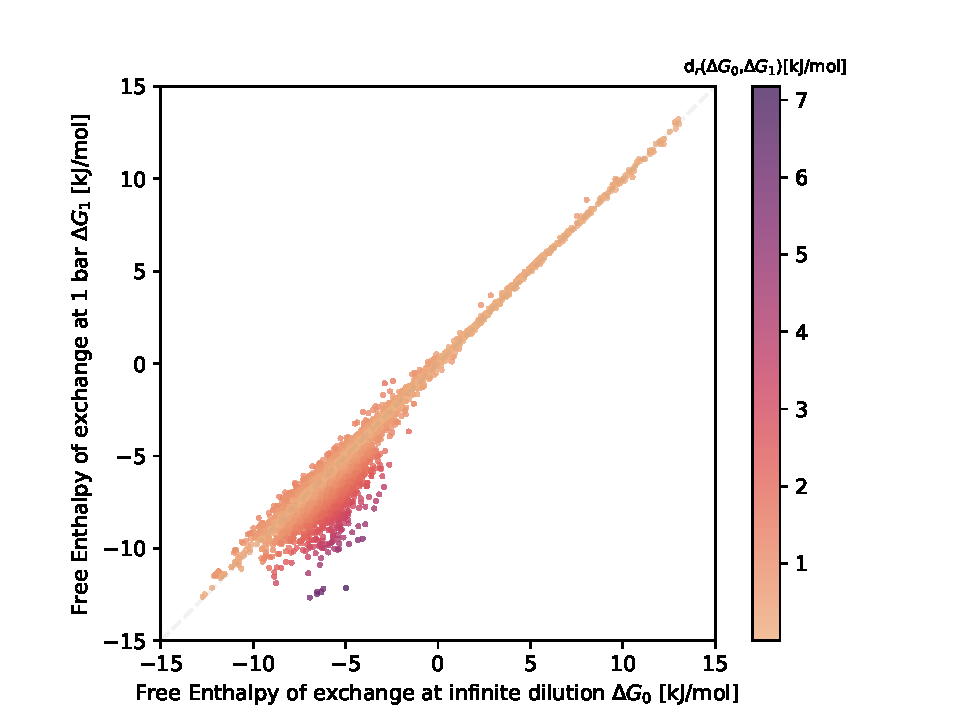
\includegraphics[width=0.5\linewidth]{figures/4-ml/main/Scatterplot_G1_G0.pdf}
  \caption{Comparison between the Gibbs free energy of exchange at low pressure $\Delta G\e{0}$ and ambient pressure $\Delta G\e{1}$ labeled by the relative distance between them. This plot is equivalent to a logarithmic plot of the selectivity at these two pressure conditions.}
  \label{fgr:problem}
\end{figure}

%% Pore size distribution & statistical descriptors
To incorporate information on the pore size diversity of the materials, I carried out statistical measurements on the PSD. By analyzing them, I detected explanatory factors at the origin of the observed selectivity drop. A high degree of multi-modality in the distribution would mean a diverse set of pores, which can lead to a selectivity drop if the pores are significantly different one from another. The more distant is the average pore size from the largest cavity diameter the higher the chance of observing a selectivity drop, because a big difference between the pore sizes bring about a lower selectivity. All these statistics are designed to give as much knowledge as possible on a hypothetical selectivity drop and on the quantitative estimation of its magnitude.

%% Energy descriptors statistics
To better quantify the change of selectivity, it could be interesting to give statistics on the distribution of interaction energies for xenon and krypton calculated by our grid algorithm. These statistics include moments of different orders (up to 4) of the energy distribution, which informs on the adsorbate--adsorbent interaction energies in the nanopores at higher loading. The shape of the energy distribution can help assess quantitatively the change in selectivity. We can consider this as a way of compressing the whole energy distribution into a few statistical values, which is a standard method used in the field of data science to tackle distribution data. The same approach has also been applied to the Boltzmann weighted distributions to generate temperature specific descriptors for the energy distributions. All these quantities have calculated and compared to the ambient-pressure selectivity in the previous chapter (section~\ref{sct:grid}).

%% 900K gaps
As explained in the previous chapter, Boltzmann averaging at higher temperature gave better result in describing the ambient-pressure selectivity description. 
This new type of descriptor is very interesting since it better performs around the high selectivity region, where the standard Boltzmann average at \SI{298}{\kelvin} loses its accuracy (see Figure~\ref{fgr:H_900K}). I used this descriptor to build several descriptors presented in the Table~\ref{tab:energy_descriptors}. As shown on the Figure~\ref{fgr:featimp_shap}, the exchange Gibbs free energy at \SI{900}{\kelvin} and the excess of free energy compared to the \SI{298}{\kelvin} case are the second and third most influential descriptors of our ML model. They are complementary to the exchange Gibbs free energy at \SI{298}{\kelvin} to predict the selectivity at higher pressures.

%% conclusion
By combining the above-mentioned features with more standard geometrical descriptors, I trained an ML model for the ambient pressure selectivity that identifies the origins of the selectivity drop and gives promising prediction results.

\clearpage

\begin{table}[ht]
  \setlength{\extrarowheight}{1pt}
  \centering
  \begin{tabular}{|l|m{10cm}|}
  \hline
   {Feature name} &  {Description} \\
  \hline
  "ASA\_m2/cm3\_1.2"  & Volumetric surface area accessible to a nitrogen probe (\SI{1.2}{\angstrom}) in \si{\square\meter\per\cubic\centi\meter} \\
  \hline
  "delta\_VF\_18\_20"  & Difference of void fraction occupiable by a krypton (\SI{1.8}{\angstrom} radius) and a xenon  (\SI{2.0}{\angstrom} radius) probe. Always positive due to the difference of probe radii. \\
  \hline
  "PO\_VF\_2.0"  & Void fraction occupiable by a xenon probe of  \SI{2.0}{\angstrom} radius \\
  \hline
  "D\_i\_vdw\_uff298"  & Largest cavity or largest included sphere diameter (LCD). Structures atom radii are defined using the UFF forcefield\textsuperscript{1} \\
  \hline
  "D\_f\_vdw\_uff298"  & Pore Limiting Diameter (PLD) or largest free sphere diameter defined similarly to the LCD  \\
  \hline
  "pore\_dist\_mean"  & Mean value of the pore size distribution or the average pore size \\
  \hline
  "delta\_pore"  & Difference between the LCD and the average pore size: "delta\_pore" $=$ "D\_i\_vdw\_uff298" $-$ "pore\_dist\_mean" \\
  \hline
  "pore\_dist\_std"  & Standard deviation of the pore size distribution \\
  \hline
  "pore\_dist\_skewness"  & Skewness (third order standardized moment) of the pore size distribution  \\
  \hline
  "pore\_dist\_kurtosis"  & Kurtosis (fourth order standardized moment) of the pore size distribution \\
  \hline
  "pore\_dist\_neff"  & Effective number of data associated to the pore size distribution: $N\e{eff} =$ sum(weights)$^2$ $/$ sum(weights$^2$) \\
  \hline
  "pore\_dist\_modality"  & Sarle's bimodality coefficient (BC) of the pore size distribution: BC $=$ kurtosis $-$ skewness$^2$ \\
  \hline
  "C\%"  & Percentage of carbon (C) in the MOF structure \\
  \hline
  "O\%"  & Percentage of oxygen (O) in the MOF structure  \\
  \hline
  "N\%"  & Percentage of nitrogen (N) in the MOF structure  \\
  \hline
  \end{tabular}
  \caption{Description of geometrical and chemical features used in the ML model.}\label{tab:geom_descriptors}
  \end{table}

\footnotetext{\textsuperscript{1}Using the approach of Ref.~\cite{Hung_2021}}
\clearpage

  \begin{table}[ht]
  \centering
  \setlength{\extrarowheight}{1pt}
  \begin{tabular}{|l|m{10cm}|}
  \hline
   {Feature name} &  {Description} \\
  \hline
  "G\_0"  & Low-pressure Xe/Kr exchange Gibbs free energy defined using the low-pressure selectivity: \\
  & $\Delta\e{exc} G\ex{Xe/Kr} = -RT\ln{\left(s\ex{Xe/Kr}\right)}$ \\
  \hline
  "G\_Xe\_900K"  & High temperature Xe adsorption Gibbs free energy defined using the Henry's constant: \\
  & $\Delta\e{ads} G\ex{Xe} (T\e{h}) = -RT\e{h}\ln{\left(RT\e{h}\rho_fK\e{H}\ex{Xe}(T\e{h})\right)}$ \\
  \hline
  "G\_Kr\_900K"  & High temperature Kr adsorption Gibbs free energy: \\
  & $\Delta\e{ads} G\ex{Kr} (T\e{h})$ \\
  \hline
  "G\_900K"  & High temperature Xe/Kr exchange Gibbs free energy: \\
    & $\Delta\e{exc} G\ex{Xe/Kr} (T\e{h}) = -RT\e{h}\ln{\left(K\e{H}\ex{Xe}(T\e{h})/K\e{H}\ex{Kr}(T\e{h})\right)}$ \\
  \hline
  "delta\_G0\_298\_900"  & Difference of exchange free energies between the ambient temperature and high temperature: \\
  & $\Delta\e{T} H\ex{Xe/Kr} = \Delta\e{exc} G\ex{Xe/Kr} (T\e{h})-\Delta\e{exc} G\ex{Xe/Kr} (T\e{0})$ \\
  \hline
  "delta\_H0\_Xe\_298\_900"  & Difference of Xe adsorption enthalpy between the ambient temperature and high temperature: \\
  & $\Delta\e{T} H\ex{Xe} = \Delta\e{ads} H\ex{Xe} (T\e{h})-\Delta\e{ads} H\ex{Xe} (T\e{0})$ \\
  \hline
  "delta\_TS0\_298\_900"  & Difference of exchange entropic term between the ambient temperature and high temperature: \\
    & $\Delta\e{T} \left(-T\Delta\e{exc}S\ex{Xe/Kr}\right) = \Delta\e{T} \left(\Delta\e{exc}G\ex{Xe/Kr} - \Delta\e{exc}H\ex{Xe/Kr}\right)$ \\
  \hline
  "enthalpy\_std\_xenon"  & Standard deviation of the Boltzmann weighted Xe energy distribution \\
  \hline
  "enthalpy\_std\_krypton"  & Standard deviation of the Boltzmann weighted Kr energy distribution \\
  \hline
  "enthalpy\_skew"  & Skewness of the Boltzmann weighted Xe energy distribution \\
  \hline
  "enthalpy\_modality"  & Bimodality coefficient of the Boltzmann weighted Xe energy distribution \\
  \hline
  "mean\_grid\_xenon"  & mean value of the xenon interaction energy distribution \\
  \hline
  "mean\_grid\_krypton"  & mean value of the krypton interaction energy distribution \\
  \hline
  "std\_grid\_xenon"  & standard deviation of the xenon interaction energy distribution \\
  \hline
  "std\_grid\_krypton"  & standard deviation of the krypton interaction energy distribution \\
  \hline
  \end{tabular}
  \caption{Description of the 15 energy-based features used in the ML model. Thermodynamic descriptors are always defined at low pressure since they are derived from an interaction energy grid. Temperatures are defined as follows: T\e{0}=298~\si{\kelvin} and T\e{h}=900~\si{\kelvin}. All these energy values are defined in \si{\kilo\joule\per\mole}.}\label{tab:energy_descriptors}
  \end{table}
  
  \clearpage

\subsection{Model training}

\subsubsection{The machine learning model}

I chose to use eXtreme Gradient Boosting (XGBoost) as the machine learning framework for our predictive model because of its accuracy, efficiency and simplicity of use. Its performance has long been proven since 17 out 29 Kaggle Challenge winning solutions were based on this algorithm in 2015. The XGBoost system is highly scalable and parallelized, which gives very fast model training.\autocite{chen2016xgboost} Compared to more standard tree-based algorithms such as random forest (commonly used in the field~\autocite{Simon_2015}), the boosting component of the algorithm means that it learns from previous mistakes and puts more efforts on the problematic data points, hence improving the accuracy of the final ML model.

In the next sections, I will introduce new descriptors for nanoporous materials, as well as new concepts of feature engineering based on energy and pore size histograms. The ML features presented have been selected by progressively filtering out the less influential ones on the accuracy of the final model, see the complete list in Table~S1-3 of Supporting Information (SI). The influence or importance is defined later in a section dedicated to the interpretation of the model. The hyperparameters of the model were fine-tuned using random searches to design the best performing final model. Finally, the influence of the preselected descriptors on the final model is interpreted using a unified approach.

\subsubsection{Hyperparameter optimization}\label{sct:hyperparameter}

A hyperparameter search consists in finding the best model to optimize the generalization error as defined in equation~\ref{eq:generalization_error}. To do so, the most common strategy consists in doing cross-validations to evaluate different model configurations. This process is called the hyperparameter search or optimization. Here, I used the randomized search algorithm to find the best parameters within a predefined reasonable range of parameters. The Python code below allowed us to find a set of optimal hyperparameters (please refer to Table~\ref{tab:hyperparameter} for the meaning of the parameters) for our final ML model.

\begin{lstlisting}[language=Python]
import xgboost as xgb
from sklearn.model_selection import RandomizedSearchCV

xgbr = xgb.XGBRegressor()
params = {
           'n_estimators': [1500],
           'max_depth': [5,6],
           'learning_rate': [0.02,0.04,0.06,0.08],
           'colsample_bytree': np.arange(0.6, 1.0, 0.05),
           'colsample_bylevel': np.arange(0.6, 1.0, 0.05),
           'alpha': np.arange(0, 4, 0.2),
           'subsample': np.arange(0.6, 0.95, 0.05),
         }
clf = RandomizedSearchCV(estimator=xgbr,
                         param_distributions=params,
                         scoring='neg_mean_squared_error',
                         n_iter=30000,
                         verbose=1)
clf.fit(X_train, y_train.to_numpy())
print("Best parameters:", clf.best_params_)
print("Lowest RMSE: ", np.sqrt(-clf.best_score_))
\end{lstlisting}

I used the training data to perform a random search of hyperparameters, with a 5-fold cross-validation to evaluate the root mean squared errors (RMSE) of the model.
After 30,000 iterations in the hyperparameter space defined by the ranges above, I found a set of optimal hyperparameters that gives an average RMSE of \SI{0.36}{\kilo\joule\per\mole} to be used in our final model.

\begin{lstlisting}[language=Python]
  optimal_params = {
      'objective':'reg:squarederror',
      'n_estimators': 1500,
      'max_depth': 6,
      'colsample_bytree':0.85,
      'colsample_bylevel':0.65,
      'subsample':0.7,
      'alpha': 0.4,
      'lambda' :1,
      'learning_rate': 0.04,
      }
  \end{lstlisting}

To confirm the relevance of the model, I performed another 5-fold cross-validation to obtain a convergence plot of the XGBoost model with this set of parameters shown in Figure~\ref{fgr:convplot}. Given this configuration, the model is tested on the prior defined test-set and interpretation tools are used to better understand the structure-property relationships in play.

\begin{figure}[ht]
  \centering
    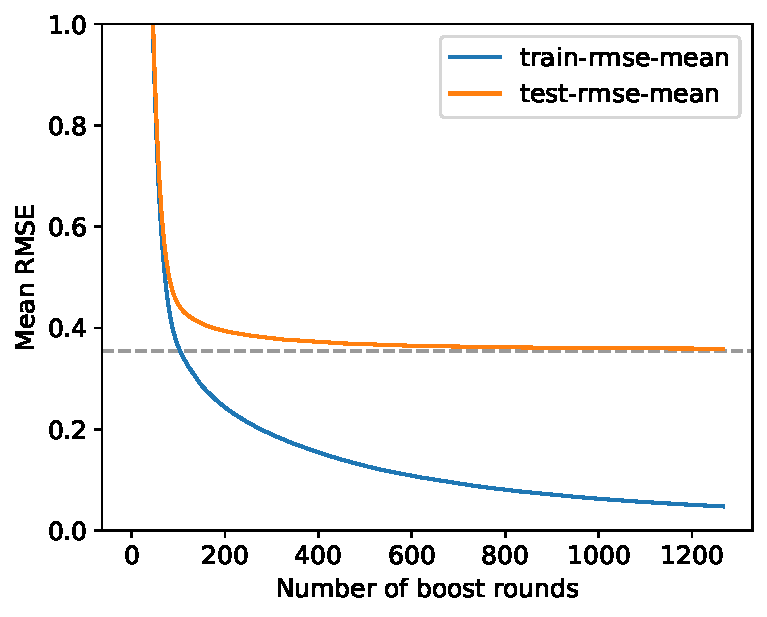
\includegraphics[width=0.60\linewidth]{figures/4-ml/SI_figure/convergence_plot.pdf}
    \caption{Convergence plot of the cross-validation training of our ML model. limit value: 0.36~\si{\kilo\joule\per\mole}}\label{fgr:convplot}
  \end{figure}

\subsection{ML model performance}

%% introduction
In this section, I will present the performance of the ML model that learned the joint effects of all the newly introduced descriptors to detect and evaluate the observed drop between the easily accessible low-pressure selectivity and the more computationally demanding ambient-pressure selectivity.
A GCMC simulation of a 20–80 xenon/krypton gas mixture takes in average \SI{2,400}{\second} per structure on the CoRE MOF 2019 database, while our grid-based adsorption calculation only takes about \SI{5}{\second} per structure (on a single Intel Xeon Platinum 8168 core at \SI{2.7}{\giga\hertz}). To compute all features needed for our prediction, we would need less than a minute per structure, which is way faster than the 40 minutes required for a GCMC calculation. The ML-based approach has a very clear speed advantage over standard molecular simulations. But to be a good substitute, it needs to keep a good level of accuracy on an unseen set of structures.

\begin{figure}[ht]
\centering
  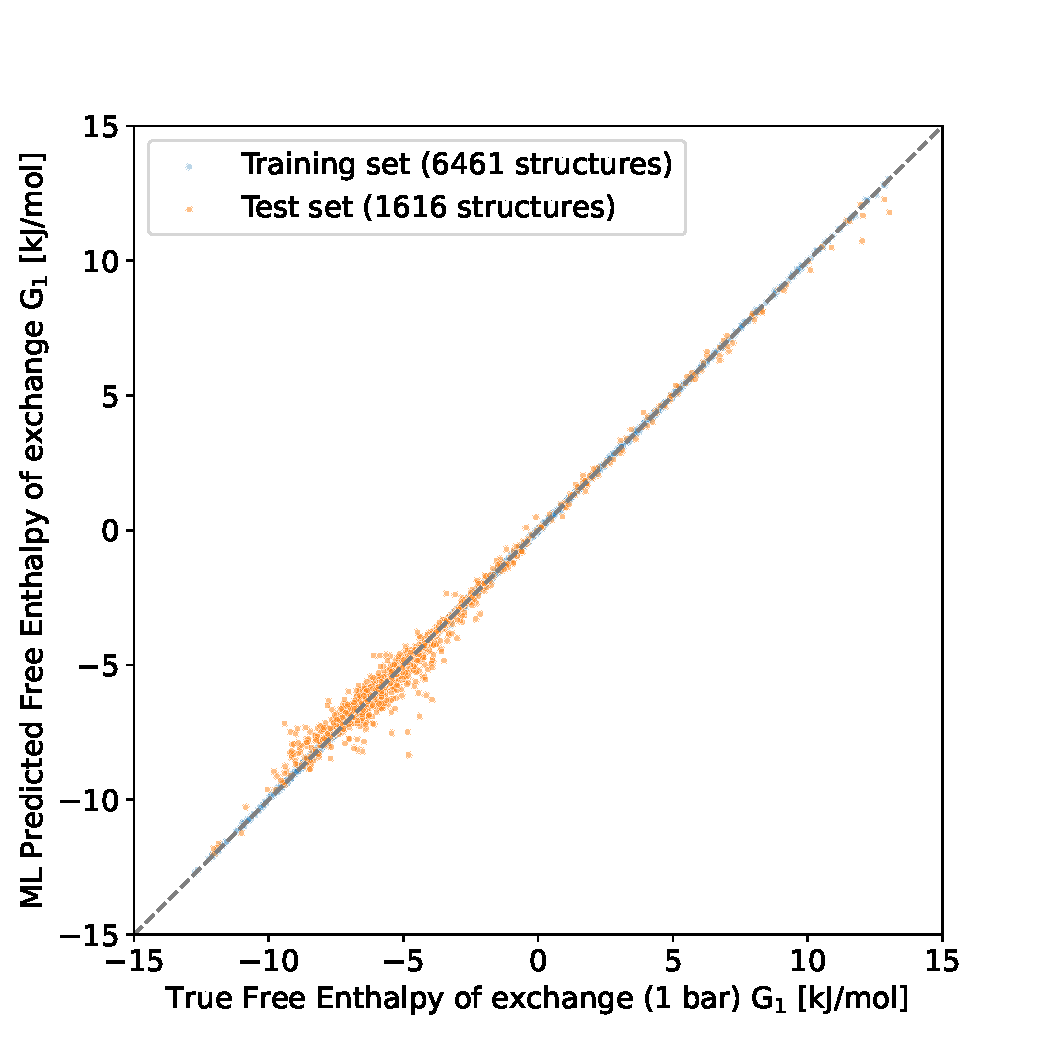
\includegraphics[width=0.5\linewidth]{figures/4-ml/main/Scatterplot_G1_prediction.pdf}
  \caption{Scatter plot of the exchange free energy predicted by the model. There is a good agreement between the predicted and true values. On the test set, there is an RMSE of \SI{0.37}{\kilo\joule\per\mole} and an MAE of \SI{0.21}{\kilo\joule\per\mole}. This plot is equivalent to the scatter plot between the logarithm of the ambient-pressure selectivity (see Figure~\ref{fgr:S1_prediction}). The corresponding errors for the ambient-pressure selectivity are 2.5 and 1.1 for respectively the RMSE and MAE of the selectivity, and 0.065 and 0.038 for the RMSE and MAE of its base-10 logarithm. }\label{fgr:G1_prediction}
\end{figure}

I defined a set of {80\%} randomly chosen structures out of the final dataset to train and fine-tune the parameters of our model. A randomized search over a range of maximum depths, learning rates, sizes of feature samples used by tree and by level, sizes of data sample and alpha regularization parameters has been performed and a set of hyperparameters have been chosen to minimize the average RMSE computed using a 5-fold cross-validation. The ranges used in the randomized search as well as the final hyperparameters set are given in the section~\ref{sct:hyperparameter}. By using this parameterization, our XGBoost model has an RMSE of \SI{0.37}{\kilo\joule\per\mole} and an MAE of \SI{0.21}{\kilo\joule\per\mole} on the exchange Gibbs free energies of the test set of 1,616 structures. If we convert back these results to the selectivity values, the RMSE on the selectivity values would be 2.5 and 0.07 on the logarithm base 10 of the selectivity, which means that the order of magnitude of the selectivity is known with a very good accuracy. To prove that this good performance is not fortuitous, I used a 5-fold cross-validation procedure on the whole dataset and found an average RMSE of \SI{0.36}{\kilo\joule\per\mole} with a standard deviation of \SI{0.01}{\kilo\joule\per\mole}, which is consistent with the performance given by a standard train/test split.

\begin{figure}[ht]
  \centering
    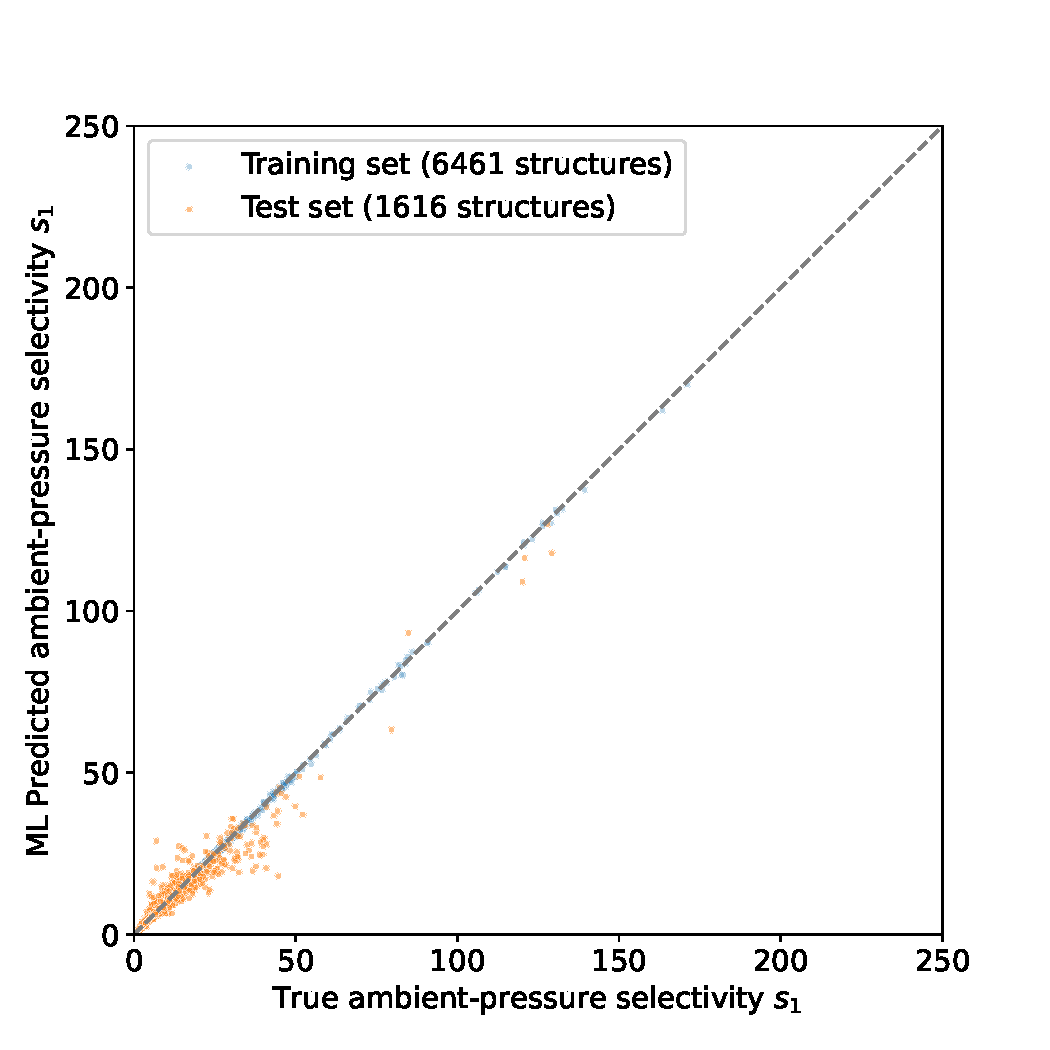
\includegraphics[width=0.48\linewidth]{figures/4-ml/SI_figure/Scatterplot_S1_prediction.pdf}
    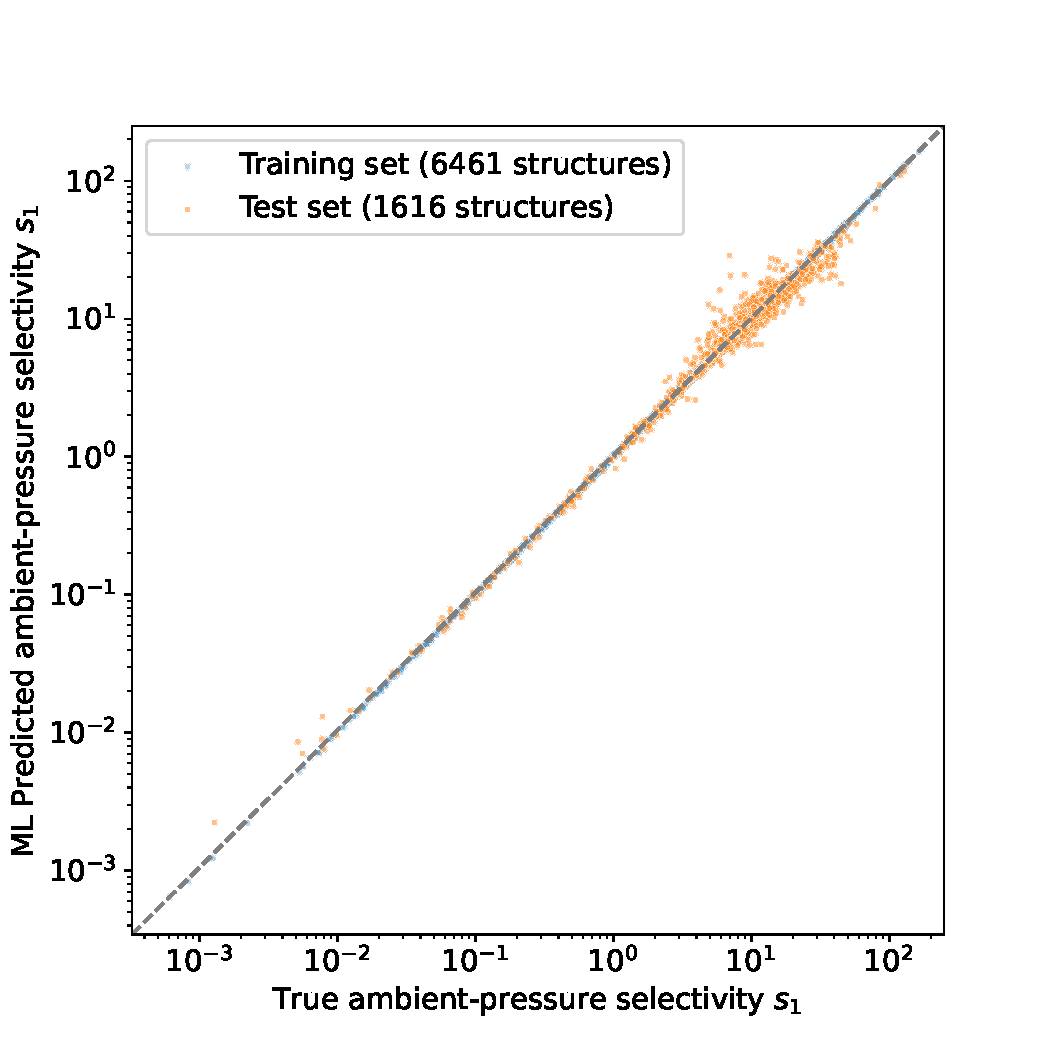
\includegraphics[width=0.48\linewidth]{figures/4-ml/SI_figure/Scatterplot_S1_prediction_logscale.pdf}
    \caption{Scatter plot of the selectivity derived by the model}\label{fgr:S1_prediction}
  \end{figure}

This method can later be used in a screening procedure that relies on cheap descriptors to skim off obviously undesirable structures to only keep the promising structures for the final ML model evaluation. For this is the reason, as previously explained in the methods, only the 3D MOF structures with an LCD above \SI{4}{\angstrom} are kept because they have a positive xenon affinity, which is a necessary condition for a good Xe/Kr selectivity. Our model being very good at predicting the ambient pressure selectivity of structures with good xenon affinity, the proposed screening procedure, illustrated Figure~\ref{fgr:pipeline}, would include (i) a check of the nature of the structure to ensure it is a 3D MOF structure, (ii) then a filter on the LCD value (above \SI{4}{\angstrom}), (iii) a pre-evaluation of the Xe/Kr selectivity at infinite dilution using the grid-based method, and (iv) finally the ML evaluation to keep only structures above a certain threshold of ambient-pressure selectivity (\emph{e.g.} 30). We could possibly evaluate more thoroughly the top structures using GCMC simulations, \emph{ab initio} calculations or adsorption experiments.

\begin{figure}[ht]
\centering
  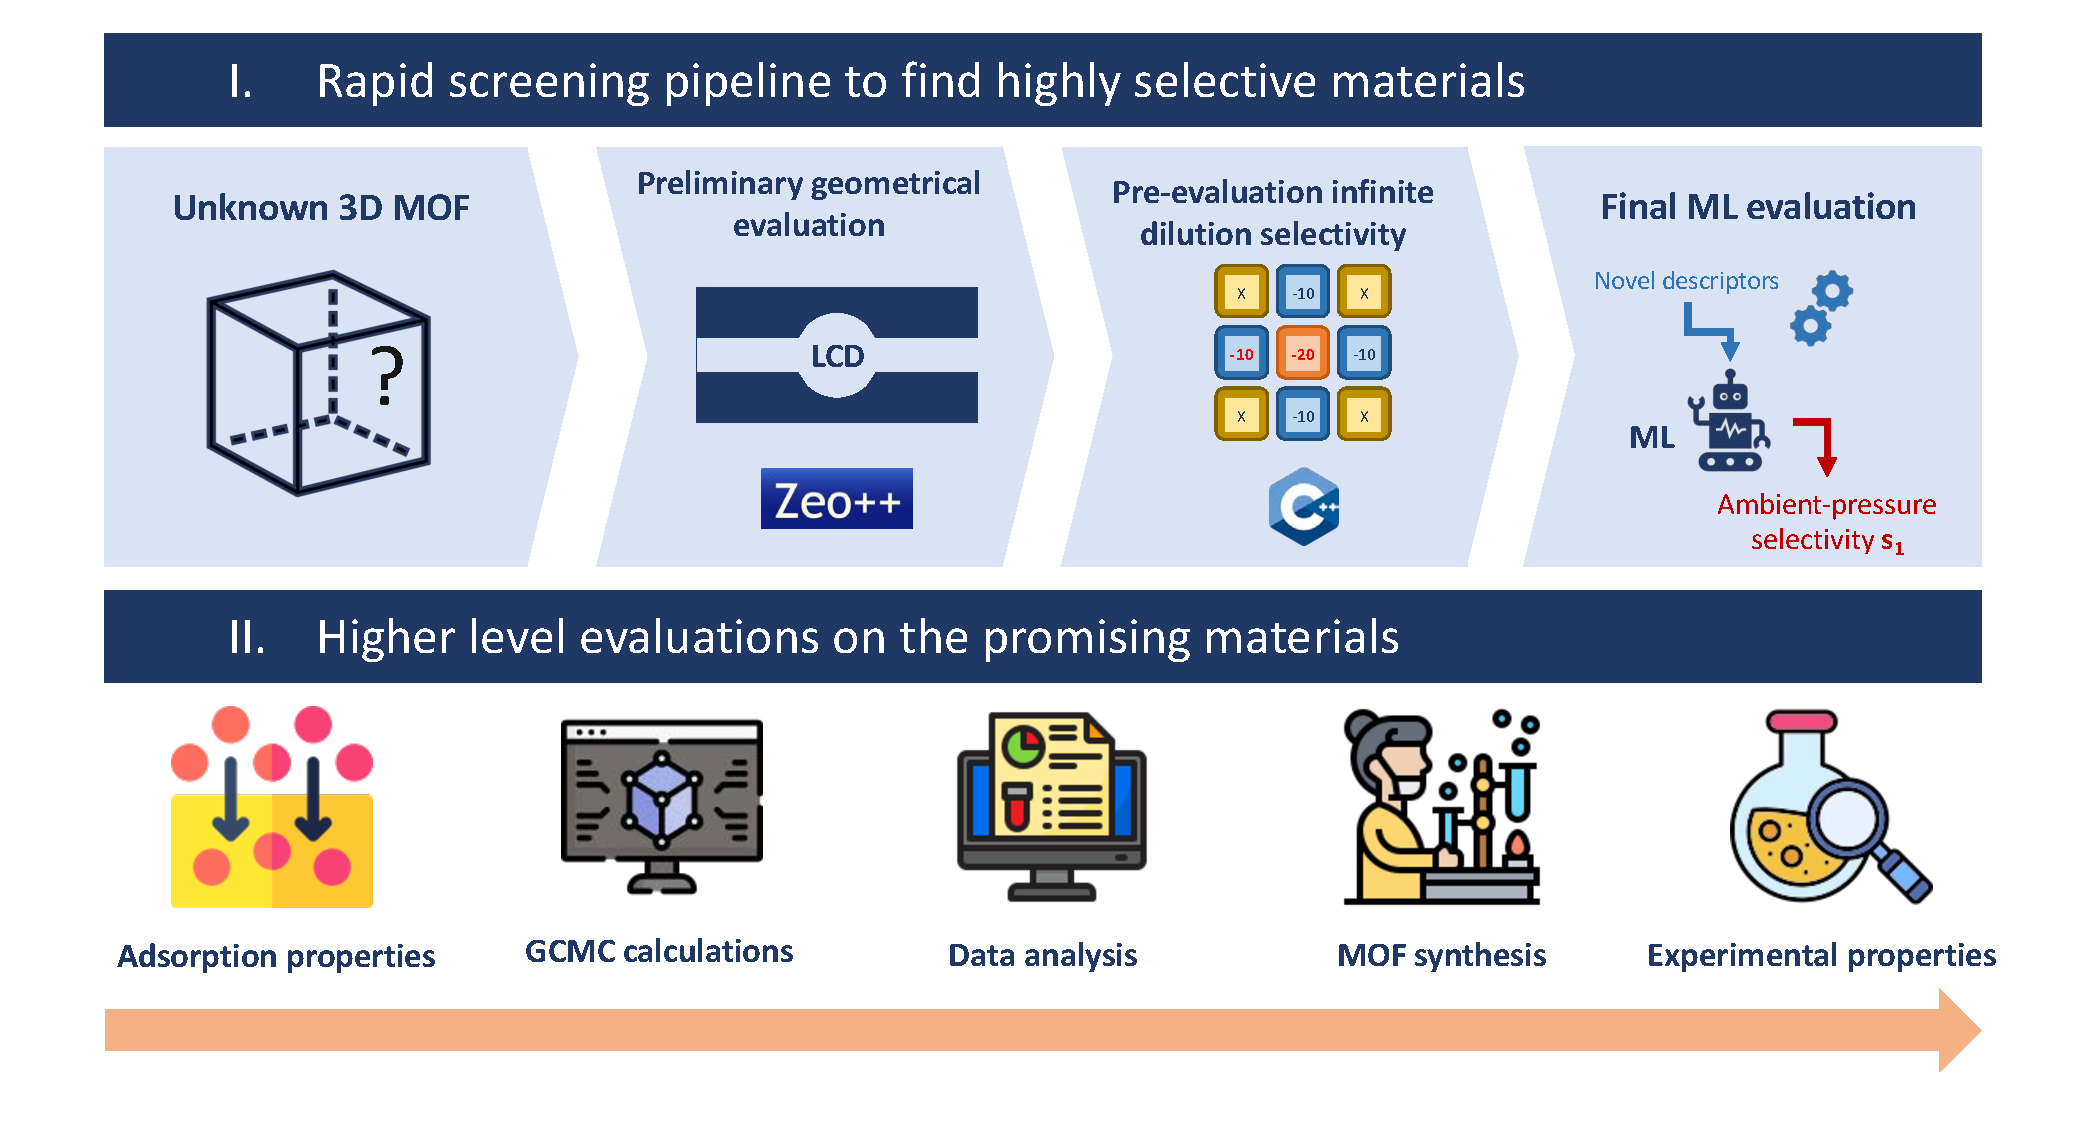
\includegraphics[width=0.99\linewidth]{figures/4-ml/main/pipeline.pdf}
  \caption{An illustration of the screening procedure that could be used to find highly selective materials.}\label{fgr:pipeline}
\end{figure}

\section{Opening the Black Box}

%% SHAP intro
To better understand the intuition behind this selectivity drop, I used the SHAP\autocite{SHAP,molnar2020interpretable} library of interpretation models to draw relationships between the descriptors and the predicted ambient-pressure selectivity. This code library is based on the calculation of Shapley values\autocite{shapley1953value} that measure the contribution of each descriptor to the prediction to locally interpret our ML model. This interpretation model untangles the interdependence between the descriptors to extract an individual contribution. To go beyond the local interpretation, we can rapidly compute the Shapley values for the whole dataset using faster algorithms;\autocite{SHAP} scatter plots of the contribution as a function of the descriptor values called SHAP dependence plots can then be drawn to make a more global interpretation of our ML model. Knowing a descriptor value, I then infer, with a certain level of uncertainty, how it changes the final predicted value, which highlights unknown structure--property relationships. Finally, I use the mean absolute Shapley values of each feature on the training set to measure the feature importance (see Figure~\ref{fgr:featimp_shap}).

\begin{figure}[ht]
  \centering
    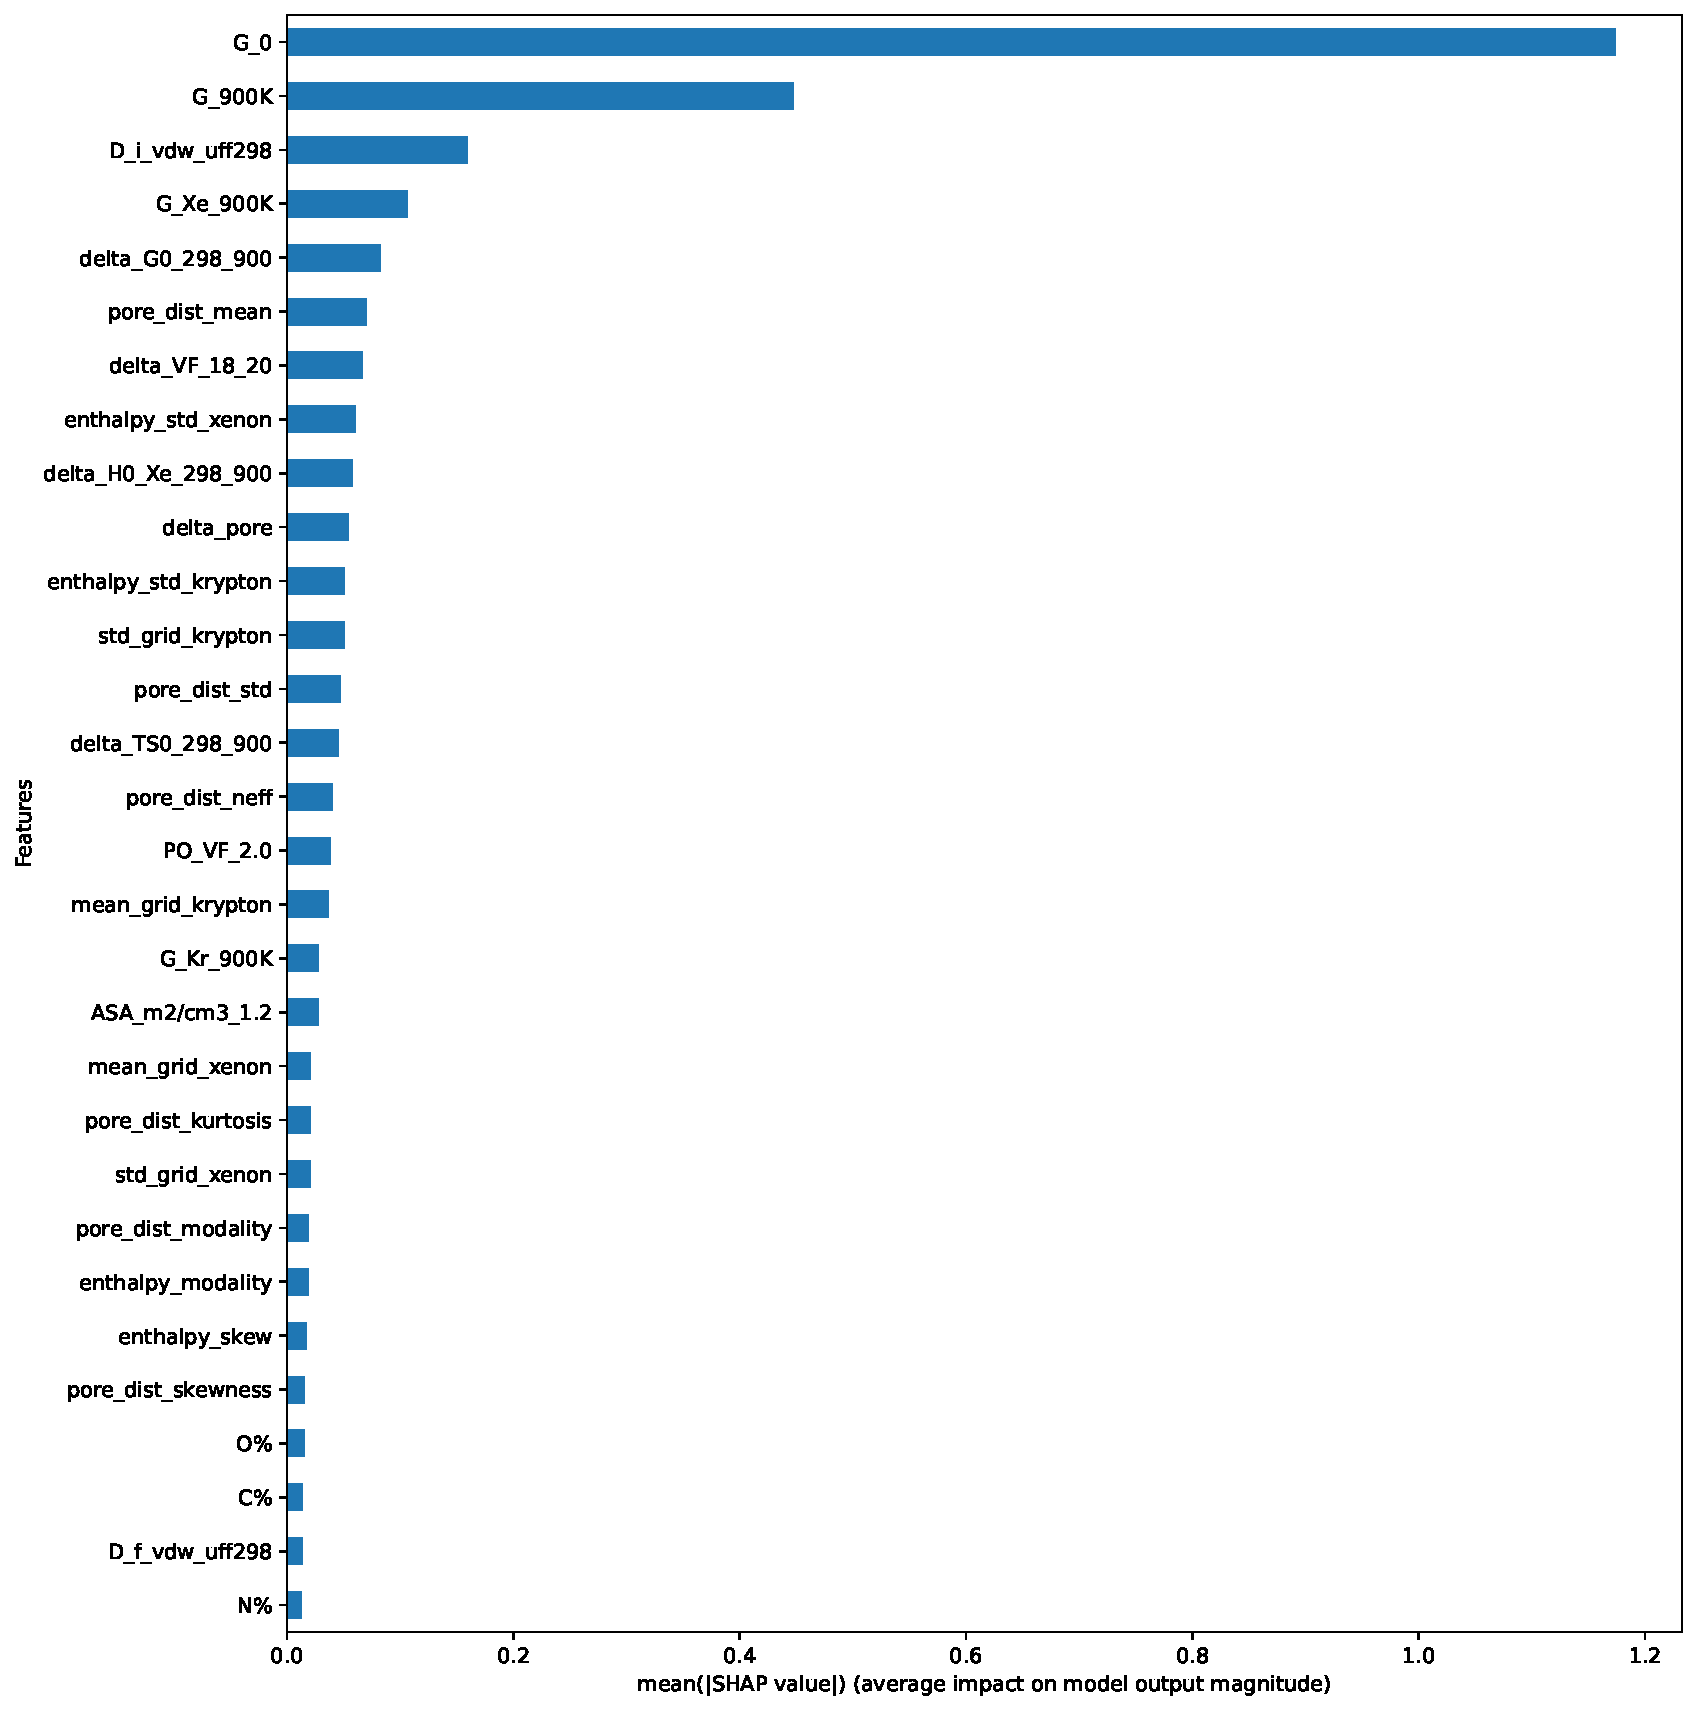
\includegraphics[width=0.70\linewidth]{figures/4-ml/SI_figure/Feature_importance_shapbased.pdf}
    \caption{Barplot of the features importance for all the descriptors of our final model. The descriptor labels used in this section are explained in more detail in Tables~\ref{tab:geom_descriptors} and \ref{tab:energy_descriptors}.}\label{fgr:featimp_shap}
  \end{figure}

\subsubsection{Explainable AI}

The final model is trained on the predefined training set using XGBoost with the fine-tuned hyperparameters. By testing it on the test set, I measured the accuracy of our approach, however, it is interesting to extract chemical insight into the hidden relationship between the predicted value and the descriptors, to better understand the thermodynamic origins of the performance. In this work, I used the Shapley values,\autocite{shapley1953value} a game theory concept developed by Shapley in 1953, to measure the contribution of each descriptor in the predicted value. This tool is used locally to understand for a given structure how their characteristics had contributed to the prediction. To draw structure-property relationships, I would need to use a global interpretation method such as the SHapley Additive exPlanations (SHAP) method thoroughly detailed in the online book \emph{Interpretable Machine Learning} of Christoph Molnar.\autocite{molnar2020interpretable} The SHAP tool developed by Lundberg and Lee~\autocite{SHAP} is based on a faster algorithm adapted to tree-based ML models like gradient boosting, TreeSHAP, and integrates useful global interpretation modules like SHAP feature importance and dependence plot.

\subsection{Global interpretability}

To rank the descriptors according to their average impact on the magnitude of the model output, I used the mean absolute Shapley values of each descriptor. The importance plot associated with these values are presented in Figure~\ref{fgr:featimp_shap}. Even if the low-selectivity exchange Gibbs free energy has a SHAP importance value way above the others, it only serves as a baseline where a correlation close to the one presented on Figure~\ref{fgr:problem} can be reached; the other descriptors play a major role in moving the outliers of the figure closer to the diagonal line. Energy descriptors play a major role in the model's prediction, and the geometry-based new descriptors, while playing a more secondary role, are key in evaluating the gaps between the low-pressure case with the ambient-pressure one that we are interested in. To dig deeper into the mechanisms that allow the model to predict the selectivity with a very good accuracy --- the RMSE and MAE on the test set's selectivity being respectively $2.5$ and $1.1$ --- I am now going to look into the SHAP dependence plots of each interesting descriptor that plots the contribution to the predicted value as a function of the actual descriptor value.

%% Global Interpretability dependence plot
To make a global interpretation, I applied the partial dependence module provided by the SHAP library on our model. Although other methods to compute dependence plots exist (\emph{e.g.} partial dependence plots),\autocite{molnar2020interpretable} we can keep a good level of consistency between our global and local interpretations by using the same underlying theory. The SHAP dependence plots of all the descriptors of the Figures~S9 and S10, these plots have a rather distinct form, directions and shape, which is encouraging for the interpretability of our model. By looking at the profile of the dependence plots, I extracted valuable information on how the ML model predicts the ambient-pressure selectivity.

%% strong relations
The most important descriptor is obviously the exchange free energy "G\_0" associated to the low-pressure selectivity, its contribution has a very strong positive linear correlation (see Figure~\ref{fgr:pdp_selection}), which gives a base value on top of which the other contributions will either reduce the free energy (more selective) or increase it (less selective). The model can be interpreted as the combination of a baseline combined with smaller tweaks that estimate the magnitude of the deviation from the ideal low dilution case. For instance, the next two descriptors "G\_900K" (\SI{900}{\kelvin} low-pressure exchange free energy) and "G\_Xe\_900K" (\SI{900}{\kelvin} low-pressure xenon adsorption free energy) continue to build up the baseline by providing information on the low-pressure selectivity, but they start giving a glimpse of deviations needed to differentiate between the structures experiencing a drop with the ones that keep their selectivity. As shown in the previous chapter (Figure~\ref{fgr:H_900K} and~\ref{fgr:G_900K}), the thermodynamic quantities at high pressure is closer to the \SI{900}{\kelvin} case than to the ambient temperature one, these two descriptors inform naturally on the selectivity at higher pressure. For "G\_900K" (see Figure~\ref{fgr:pdp_selection}), blue points (corresponding to a "G\_0" of around \SI{-8}{\kilo\joule\per\mole}) can have either negative or negligible contributions depending on the value; values below \SI{-4}{\kilo\joule\per\mole} give a negative contribution with a linear relation, whereas values between $-4$ and \SI{5}{\kilo\joule\per\mole} give constantly almost zero contributions. This type of domain differentiation illustrates how the model can identify structures with a selectivity drop based on the values of a descriptor. I will introduce more telling examples of how the contribution to the selectivity values are determined using the values of the remaining descriptors.

%% optimal values
The U-shape of some SHAP dependence plots can highlight optimal values for the associated descriptors. For instance, the optimal value of "D\_i\_vdw\_uff298" is around $5.1$ (see Figure~\ref{fgr:pdp_selection}) and the optimal average of pore sizes is around $5.6$. These optimal values match with the physical need of having pores of the size of a xenon to be more attractive to it, which was identified in several papers in the literature. These values are a bit higher than the ones mentioned in the literature due to the different definition of the atom radii.\autocite{Hung_2021} Moreover, values of "delta\_G0\_298\_900" between $4$ and \SI{6}{\kilo\joule\per\mole} (see Figure~\ref{fgr:pdp_selection}) have a higher chance of giving a negative contribution, which means a lower ambient-pressure selectivity. These sweet spots constitute valuable hints to tell the truly selective materials from the others. Some SHAP dependence plots have a rather linear domain for the most selective structures (in blue) --- the difference of pore volumes between Xe and Kr sized probes "delta\_VF\_18\_20" have a good linear contribution (see Figure~\ref{fgr:pdp_selection}), which means that a lowervoid fraction dfference would imply a more selective structure. The same can be said for the standard deviations of the PSD "pore\_dist\_std" and of the Boltzmann weighted krypton interaction energies distribution "enthalpy\_std\_krypton". The optimal values for these descriptors are zero, the closest the value gets to zero and the more negative the contribution will be, which means a more selective structure at ambient pressure.

%% optimal domains (weak relations)
Sometimes the optimal values are not around well-identified values but are contained within larger domains with threshold values separating them. For instance, the difference between the LCD and the average pore size "delta\_pore" has a threshold value around \SI{0.3}{\angstrom} below which the contribution for the most selective structures (blue) is negative (see Figure~\ref{fgr:pdp_selection}); even though no clear correlations can be found, we can at least find a threshold value (about $0.23$) below which there is higher probability of having a high ambient-pressure selectivity. The same type of domain splits can be found for the average of krypton interaction energies distribution "mean\_grid\_krypton" (at around $15$), the Boltzmann weighted xenon interaction energies distribution "enthalpy\_std\_xenon" (at around $2.5$), the difference of exchange entropic term between the ambient temperature "delta\_TS0\_298\_900" (at around $3$) and high temperature and the effective number associated to the PSD "pore\_dist\_neff" (at around $2.3$). These domains separate structures that are selective at low pressure, which is key to telling apart the structures with a selectivity drop at ambient pressure from the ones without.

\begin{figure}[ht]
\centering
  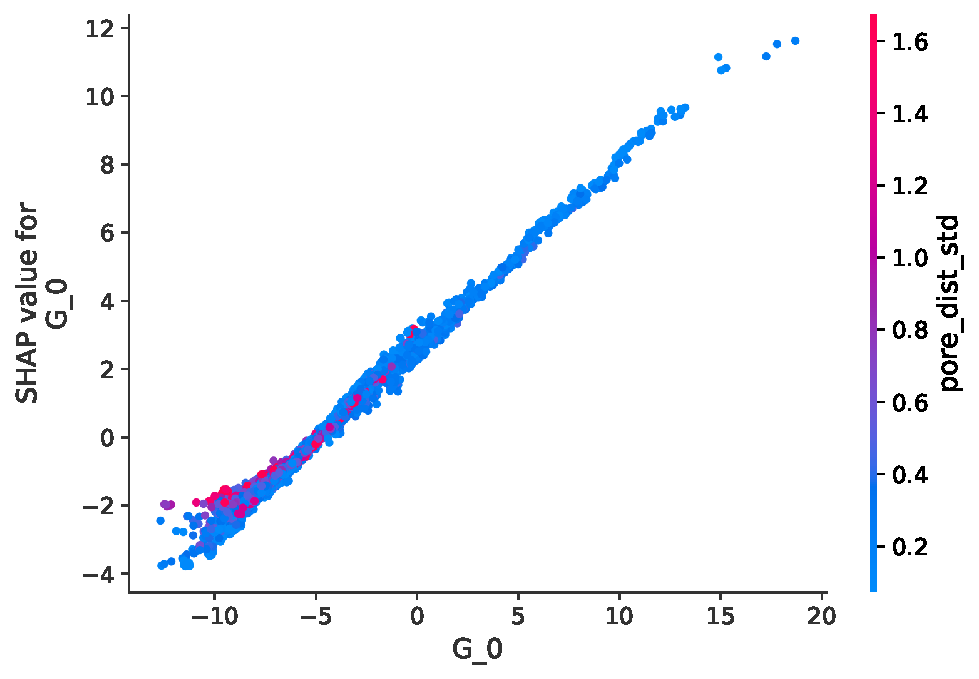
\includegraphics[width=0.32\linewidth]{figures/4-ml/SDP/G_0.pdf}
  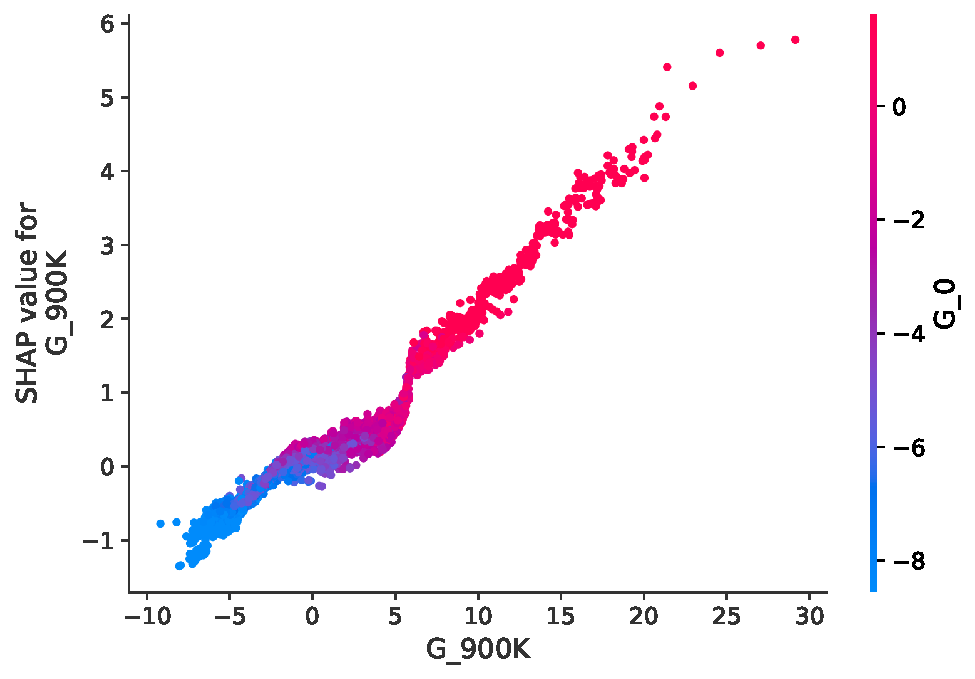
\includegraphics[width=0.32\linewidth]{figures/4-ml/SDP/G_900K.pdf}
  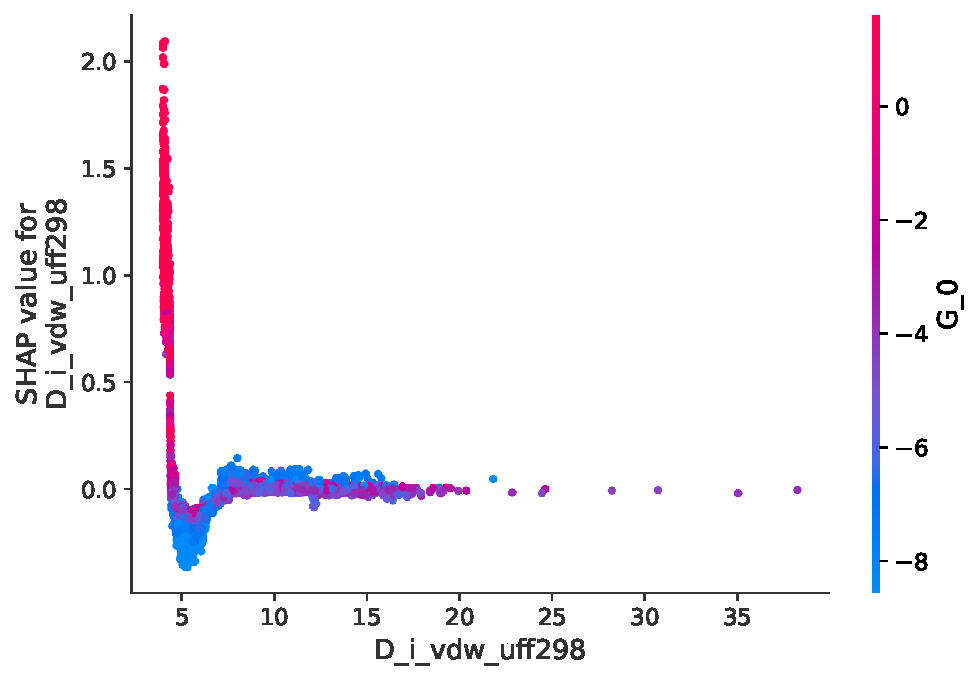
\includegraphics[width=0.32\linewidth]{figures/4-ml/SDP/D_i_vdw_uff298.pdf}
  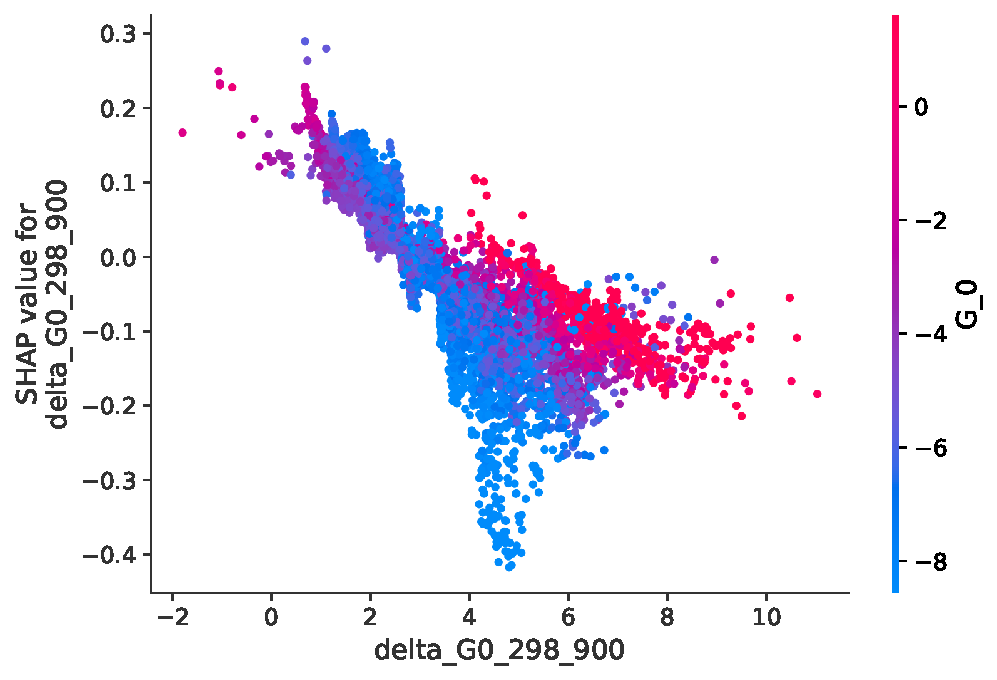
\includegraphics[width=0.32\linewidth]{figures/4-ml/SDP/delta_G0_298_900.pdf}
  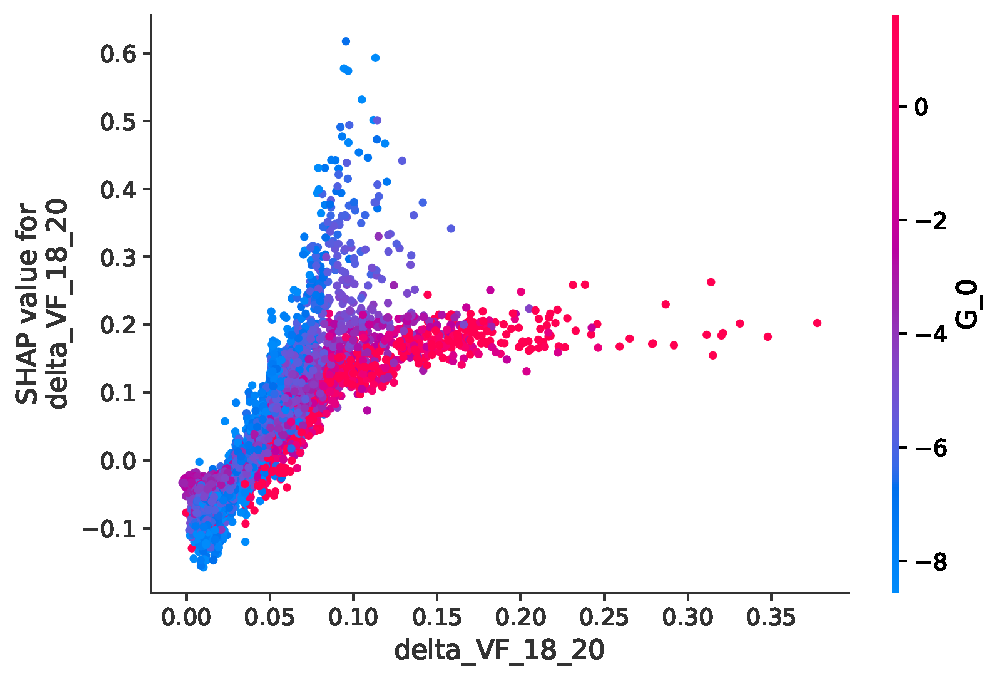
\includegraphics[width=0.32\linewidth]{figures/4-ml/SDP/delta_VF_18_20.pdf}
  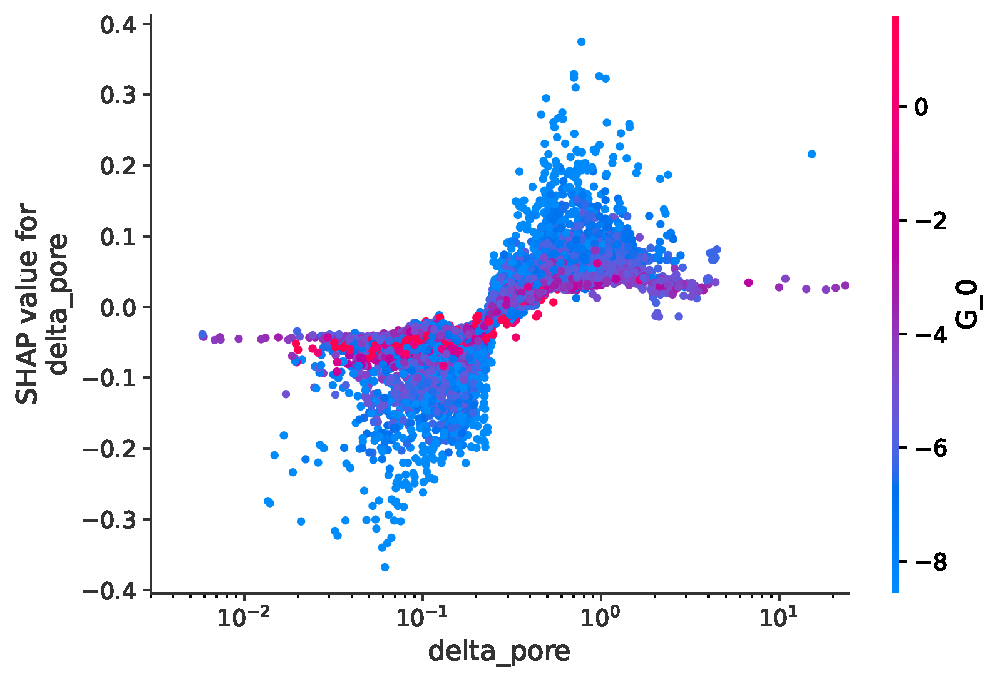
\includegraphics[width=0.32\linewidth]{figures/4-ml/SDP/delta_pore.pdf}
\caption{Some SHAP dependence plots that are analyzed here.}\label{fgr:pdp_selection}
\end{figure}

\subsection{Local interpretability}

%% local interpretation
To put into practice our previous analysis, let's look at some archetypal structures and how the model predicted the selectivity based on the descriptor values. I chose two MOF structures from the test set, their CSD code being respectively VIWMIZ and BIMDIL. Both structures are selective at low pressure but the first one decreases in selectivity while the other maintains it at ambient pressure. It will be interesting to see what the model does to tell apart these two completely different behaviors.

VIWMIZ is part of the highly selective structures that experience a selectivity drop at ambient pressure. If I convert back the free energy values to selectivity values, its selectivity is $62.8$ at infinite dilution and $14.5$ at ambient pressure. The ML model manages to give a close prediction of $12.0$ for the ambient-pressure selectivity based on the given values of the descriptors. If we only look at "G\_0", it has one of the most negative values, which explains the rather high negative contribution of $-1.81$. However, the $-0.57$ contribution of "G\_900K" is rather low compared to other materials (see Figure~\ref{fgr:pdp_selection}), since a value of $-4.05$ is not the most negative considering all structures. On the other hand, the remaining descriptors have values in the domain of positive contributions, which lead to the drop of the selectivity. For example, the difference of pore sizes "delta\_pore" has a value of \SI{1.38}{\angstrom} (above the threshold of \SI{0.23}{\angstrom}), which contributes $+0.25$ to the predicted selectivity and is consistent with the value ranges of the associated dependence plot. By reporting the values to the dependence plots, the same analyses can be made on the other positive contributions of the Figure~\ref{fgr:contribution}: "pore\_dist\_std" is above the threshold of $0.4$, "enthalpy\_std\_krypton" is above \SI{2.5}{\kilo\joule\per\mole}, "pore\_dist\_neff" is above $2.3$, "delta\_TS0\_298\_900" is below \SI{3}{\kilo\joule\per\mole} and "enthalpy\_modality" is around $0.75$ where positive contributions are more commonly observed. However, the "delta\_G0\_298\_900" value is a bit too close to its optimal value, which explains its negative contribution in this particular prediction. The rest of the features have almost negligible contributions. By analyzing the contributions of each descriptor to the prediction given by our model, we can understand the underlying features of the VIWMIZ structure that explains the selectivity drop at higher pressure. The shape of the xenon and krypton energy distributions ("enthalpy\_std\_krypton" and "enthalpy\_modality") and of the PSD ("pore\_dist\_std" and "pore\_dist\_neff" ) as well as the void fraction difference "delta\_pore" are key descriptors at the origin of the lower selectivity at ambient pressure compared to the ideal infinite dilution case. Intuitively, one can easily understand that effective number of pores exceeding 2 can mean the presence of different pore sizes, which is consistent with the presence of pores that are less attractive to the xenon and leads necessarily to less selectivity. The previous statement is also very much consistent with a high standard deviation of the PSD or the Boltzmann weighted krypton interaction energy distribution. One can also conceive that a much larger difference between the average pore size and the LCD could mean a high disparity in pore sizes that leads to the presence of larger pores more and more loaded as the pressure rises.
The entropic term is, however, way more complex to interpret and opens unexplored ways of tackling the problem of selectivity drop at higher pressure unraveled by our previous study (chapter 2).

\begin{figure}[ht]
    \centering
    \begin{subfigure}[b]{0.47\textwidth}
      \centering
      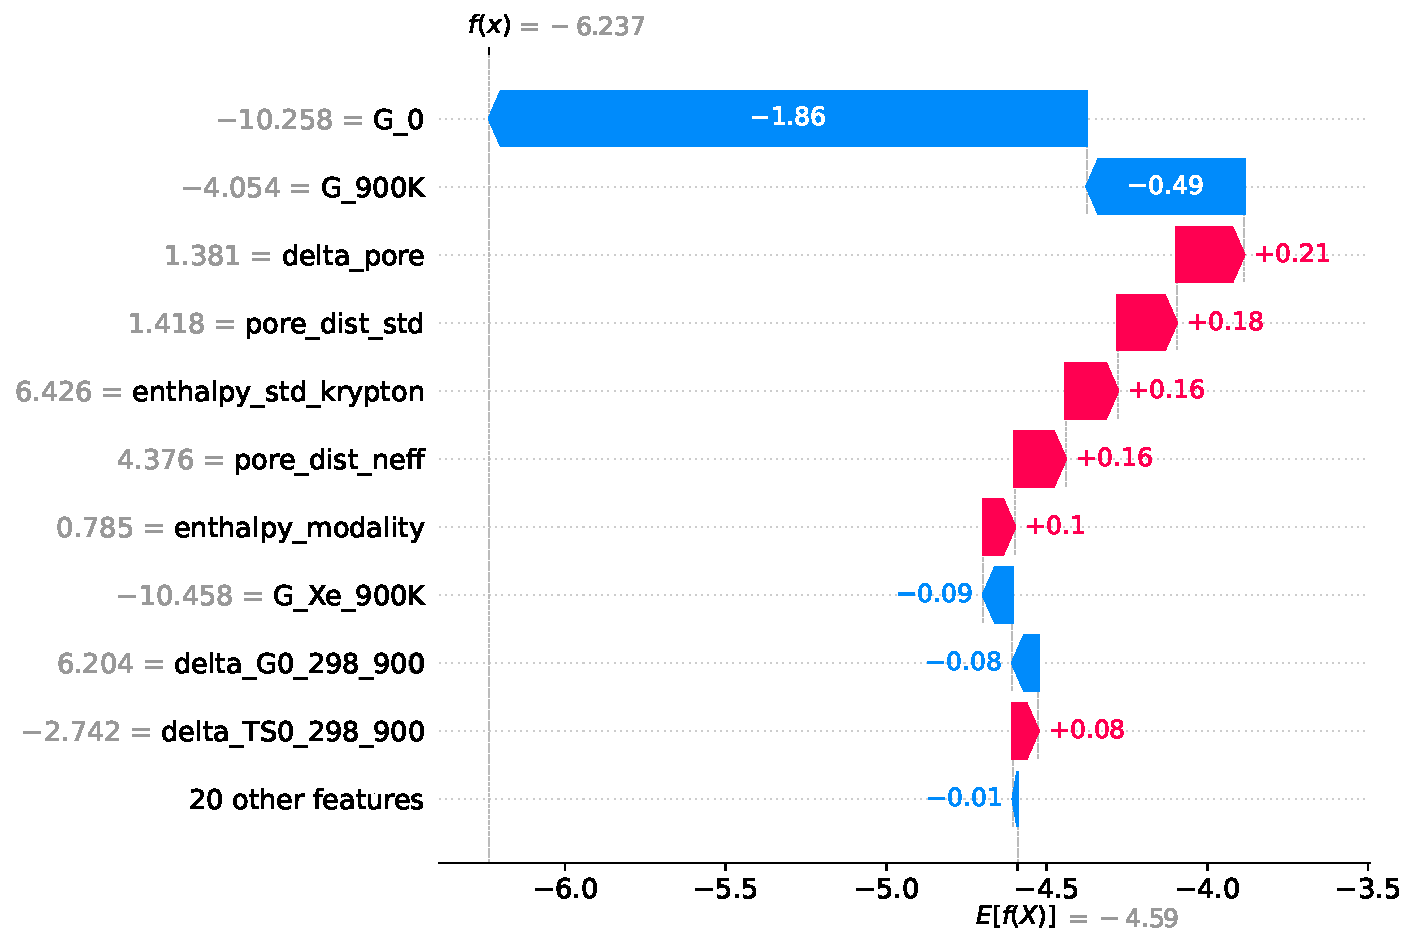
\includegraphics[width=\textwidth]{figures/4-ml/main/VIWMIZ_clean.pdf}
      \caption{VIWMIZ: true $\Delta\e{exc} G_1=-6.63$}
    \end{subfigure}
         \hfill
    \begin{subfigure}[b]{0.47\textwidth}
      \centering
      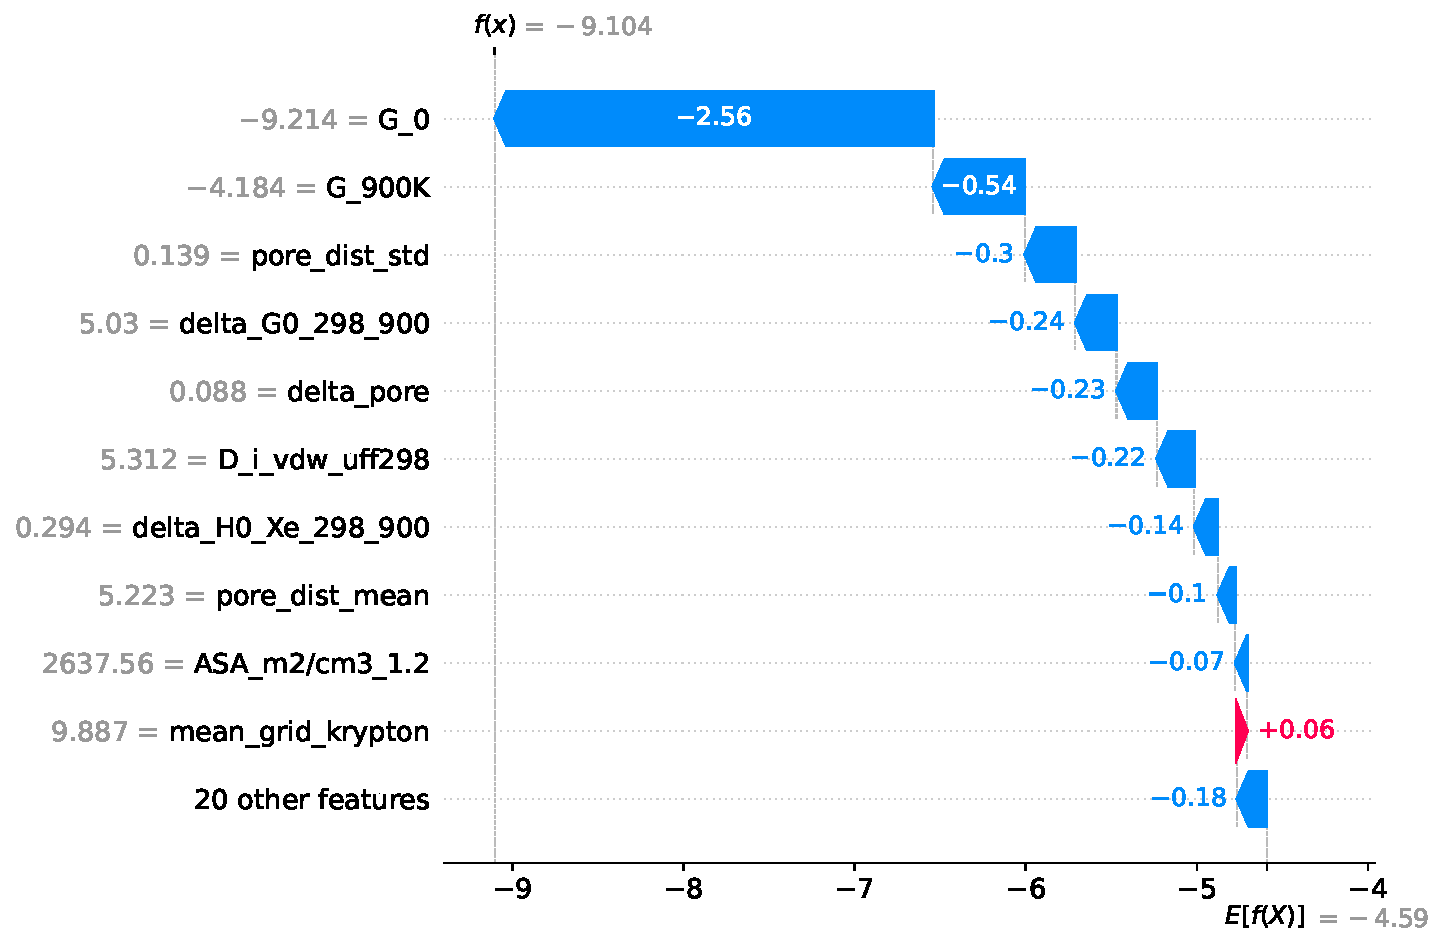
\includegraphics[width=\textwidth]{figures/4-ml/main/BIMDIL_clean.pdf}
      \caption{BIMDIL: true $\Delta\e{exc} G_1=-9.20$}
    \end{subfigure}
  \caption{Main contributions of the descriptors on the selectivity prediction of two archetypal examples. The descriptor labels used are detailed in the Table~\ref{tab:geom_descriptors} and~\ref{tab:energy_descriptors}.}\label{fgr:contribution}
\end{figure}

The second structure BIMDIL is also among the most selective with a selectivity at low pressure of $41.0$, while maintaining it to $41.2$ at ambient pressure. The model manages to predict this stability of the selectivity by giving a value of $40.0$. Consequently, the first contribution of "G\_0" is among the most negative ones and set a baseline of $-2.4$ for the upcoming contributions. The contributions of "G\_900K" and "G\_900K" are not the highest possible but they continue to lower down the value of the predicted selectivity. It is the joint contributions of the other descriptors that will really discriminate between the two structures and decide why this one will keep its selectivity. Unlike the previously analyzed structure, this one has a "delta\_pore" value below \SI{0.3}{\angstrom}, which explains the negative Shapley value it has for our prediction. The contribution of "delta\_G0\_298\_900" that was only a little negative for the other one, is now playing a major role since it is right within the range of between $4$ and \SI{6}{\kilo\joule\per\mole} (see Figure~\ref{fgr:contribution}). We can also verify that "pore\_dist\_std" is now below the threshold instead of being above for the other structure. We can confirm that the other contributions are also following the rules implied by the SHAP dependence plots, no apparent anomalies are detected, and the joint efforts of all the descriptors tend to give a lower free energy value, which leads to the conservation of the selectivity value at higher pressure. The set of descriptor values is clearly very different from the previous structure, many values are in opposite contribution domains, which explains how the model manages to disentangle the highly selective structures to find out the ones that would keep their selectivity at higher pressure.

%% conclusions + sum-up of some qualitative rules
These two examples allow us to understand fairly more how the model tells apart the structures that will lose selectivity at higher pressure from the ones that will not. Most of the dependence plots can give very strong association between the descriptors and their effects; the outliers are rare enough that the inner logic of our model can be understood. As developed previously, the first three descriptors set a baseline on the observed selectivity drop with reasonably little information; then the other descriptors contribution is either positive, negligible or negative depending on the domain of values the descriptor is in. For instance, the average pore size and the largest cavity diameter need to be around very specific values to maximize the chance of keeping the selectivity at higher pressure, which was highlighted by previous works that emphasize on the importance of pore sizes close to the size of xenon for Xe/Kr separation. The difference of entropy between the ambient temperature and \SI{900}{\kelvin} is surprising descriptor that separates selective structures depending on whether its value is within a given range. The difference of void fraction occupied by xenon and krypton is also very interesting since it impacts the selectivity differently depending on whether it is highly selective or not, and the contribution is more or less proportional to its value. Different ways of measuring the disparity of the PSD and interaction energy distribution are key in sorting highly selective structures (in blue on the dependence plot Figure~\ref{fgr:pdp_selection}) between the ones maintaining their performance and the ones decreasing in selectivity. Among others, we can find the difference between the average pore size and the LCD, as well as the standard deviation of the PSD or of the Boltzmann weighted energy distribution that would behave very differently according to the domain in which the value lies. The SHAP dependence plots are very valuable reading grid to understand the mechanisms behind our ML model and more broadly to what it understood from the origins of Xe/Kr separation.

\textbf{Data Availability:} \url{} \todo{create a repo github with the different models and data}

\section{Beyond thermodynamic considerations}

In order to better understand separation processes inside nanoporous materials, I performed a machine learning prediction of Xe/Kr ambient-pressure selectivity that is faster than standard GCMC calculations. For MOF structures of the CoRE MOF 2019 database, a xenon/krypton selectivity evaluation would take less than a minute, while an equivalent GCMC calculation takes around \SI{40}{\minute}. Unlike most of the selectivity predictions of the literature, I chose to predict a selectivity in the logarithmic scale, because it focuses more on the order magnitude than the exact value of the selectivity of highly selective materials. Moreover, the conversion to an exchange Gibbs free energy allows a more thermodynamic approach based on enthalpy, entropy and free energy values. The challenge was then to predict a free energy equivalent of the ambient-pressure selectivity by using the low-pressure selectivity along with key energy, geometrical and chemical descriptors. The final, fully optimized ML model performs very well with an RMSE of \SI{0.36}{\kilo\joule\per\mole}, which corresponds to a $0.06$ RMSE on the base-10 log of the selectivity.

One of our more specific goals was to uncover underlying reasons of a selectivity drop at high pressure observed on some highly selective materials at low pressure. Previous studies (chapter 2) found that a high diversity of pore sizes and channel sizes that favor adsorbate reorganizations could be at the origin of this phenomenon. By applying interpretability tools, I found quantitative factors that explain the conservation or the drop of the selectivity for highly selective materials. Depending on energy averaging at \SI{900}{\kelvin}, on statistical characterizations of the energy or pore size distributions, and on the difference of volumes occupiable, a structure can either exhibit a selectivity similar to the infinite dilution case or that is much lower at higher pressure. All the quantitative rules are contained in a complex ensemble of decision trees constructed by our XGBoost model, and they can be extracted to build rule of thumbs in order to back our intuition on the Xe/Kr selectivity in MOF structures.

%% Framework could be reproduced for other type of applications
The final ML model can be used in a well-designed workflow to find the best performing materials. For instance, we could filter out the structures with pores that cannot fit a xenon in, then we could use a first calculation of the low-pressure selectivity to filter out the selectivity below a given threshold. Finally, we can use the model to remove the structures that would experience a selectivity drop. I tested our methodology on the Xe/Kr separation as proof of concept since it is one of the simplest adsorption systems (monoatomic species with no electrostatic interactions). A similar approach can be generalized to other separation applications by calculating the infinite dilution energies with a more standard method (\emph{e.g.} Widom's insertion) and by adjusting the descriptor definitions to fit the adsorbates of interest.

%% Drawbacks + perspectives
This study ambitions to add new descriptor ideas to help the development of ever more efficient screening methodologies to find the best materials for target applications. However, like many other studies on the topic, this one also relies on a few strong assumptions --- the simulations are performed in rigid frameworks with non-polarized classical force fields. As suggested in the literature, the most selective materials ever synthesized for Xe/Kr separation are all based on the effect of open-metal sites that uses the difference of polarizability between the two molecules to efficiently separate them.\autocite{Li_2019, Pei_2022} Moreover, the structures can be made flexible using flexible force fields with adapted simulation methodologies\autocite{Bousquet2012} or by using multiple rigid simulations of snapshots from NPT simulations\autocite{Witman_2017}.
It would be possible to improve the simulations at the cost of CPU times, if we coupled it with a reduction of simulation time like the one presented in this chapter. The quest of ever-faster evaluation tools will allow us to investigate more complex properties and uncover structures with ever more interesting characteristics. These potential improvements will be discussed more in depth in the chapter 6.

\vspace{1cm}

In the next chapter, I will focus on another shortcoming of the simple thermodynamic approach which is the consideration of kinetic limitations in the screening process. In our problem of adsorbent-material separation, the transport effect is not key in evaluating the separation performance of the material but is rather a constraint that could alter the performance of some seemingly top materials. Different methodologies will be explored in order to incorporate these computationally expensive and experimentally hard to get transport properties. 

\OnlyInSubfile{\printglobalbibliography}

\end{document}
